\chapter{Distributed Delay Model}

\section{Quadrature}\label{section:quad}
The integration domain $[a, b]$, with $a=\tau-n\sigma$ and $b=\tau+n\sigma$, can be discretised into $N$ sub-intervals of equal length with $N+1$ discretisation points, $s_0,\cdots,s_{N}$, such that $s_0=\tau-n\sigma$ and $s_N=\tau+n\sigma$. Using the composite Simpsons's rule \cite{compsimp}, the integral term can be numerically approximated as

\begin{equation}\label{simp}\int_{a}^{b}k(s)\hat{u}^2\hat{v}\  \text{ds}\approx\frac{h}{3}\left[k(s_0)\hat{u}^2_0\hat{v}_0+2\sum_{i=1}^{\frac{N}{2}-1}k(s_{2i})\hat{u}^2_{2i}\hat{v}_{2i}+4\sum_{i=2}^{\frac{N}{2}}k(s_{2i-1})\hat{u}^2_{2i-1}\hat{v}_{2i-1}+k(s_N)\hat{u}^2_N\hat{v}_N\right],
\end{equation}
where $h$ is computed as $h=\frac{b-a}{N}$. We use the notation $\hat{u}_j$ and $\hat{v}_j$ to denote $u(t-s_j)$ and $v(t-s_j$) respectively, namely the functions $u$ and $v$ evaluated at time-delay with some index $j$, $s_j$. Throughout the report we use $n=3$, so that the integration limits are $a=\tau-3\sigma$ and $b=\tau+3\sigma$. This was chosen so that a relatively large $\sigma$ value could be chosen for each $\tau$ while maintaining $a>0$.
Figures \ref{fig:pdf1} and \ref{fig:pdf2} show the pdf of a truncated Gaussian distribution centred at a mean $\tau=1,2$ with varying $\sigma$ values as fractions of $\sigma_{max}$. We have $s$ as the integration variable, with $s\in[a,b]$.

\begin{figure}[H]
    \centering
    \begin{subfigure}[b]{0.45\textwidth}
        \centering
        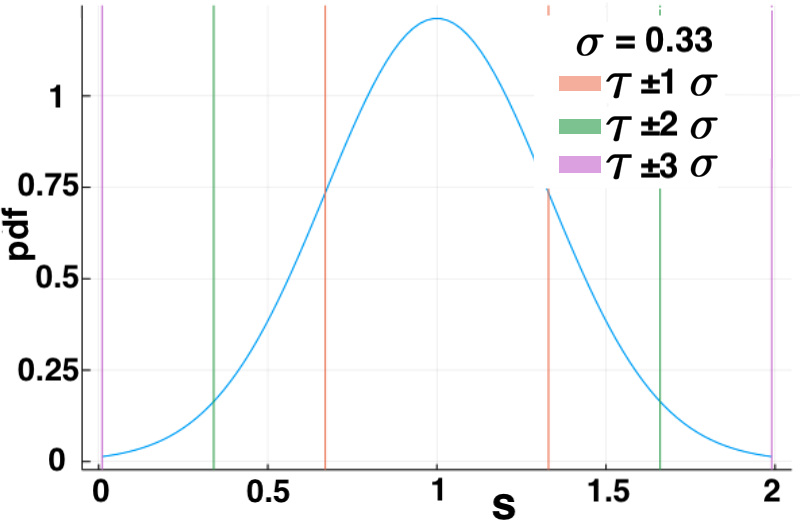
\includegraphics[width=7cm,height=5cm]{t1sig1.png}
        \caption{Truncated Gaussian distribution following $\mathcal{N}(1,(\sigma_{max}\times0.99)^2)$}
        \label{}
    \end{subfigure}
    \hfill
    \begin{subfigure}[b]{0.45\textwidth}
        \centering
        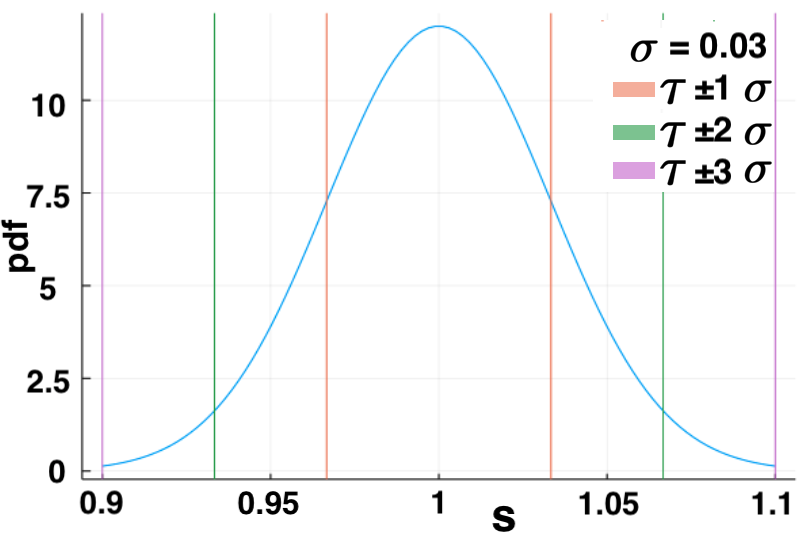
\includegraphics[width=7cm,height=5cm]{t1sig2.png}
        \caption{Truncated Gaussian distribution following $\mathcal{N}(1,(\sigma_{max}\times0.1)^2)$}
        \label{}
    \end{subfigure}
\caption{PDF of truncated Gaussian distribution with mean $\tau=1$ and integration domain $[1-3\sigma,1+3\sigma]$.}
\label{fig:pdf1}
\end{figure}
\begin{figure}[H]
    \centering
    \begin{subfigure}[b]{0.45\textwidth}
        \centering
        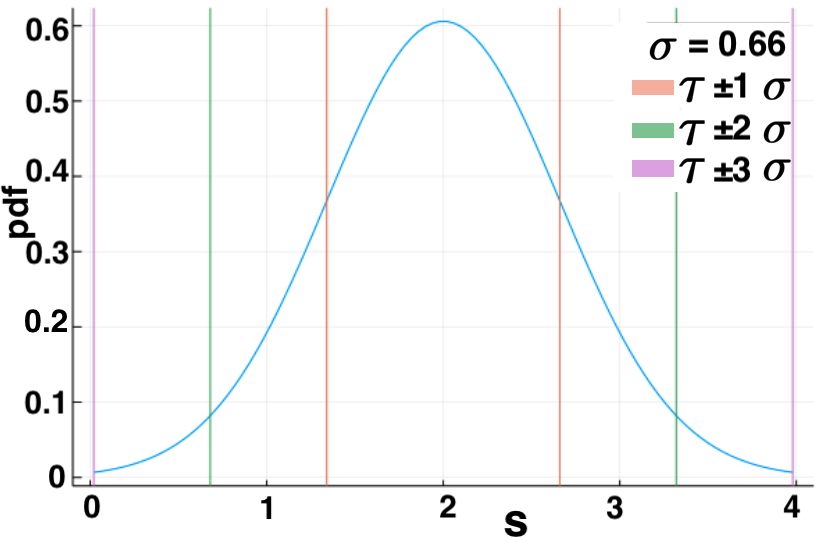
\includegraphics[width=7cm,height=5cm]{t2sig1.png}
        \caption{Truncated Gaussian distribution following $\mathcal{N}(2,(\sigma_{max}\times0.99)^2)$}
        \label{}
    \end{subfigure}
    \hfill
    \begin{subfigure}[b]{0.45\textwidth}
        \centering
        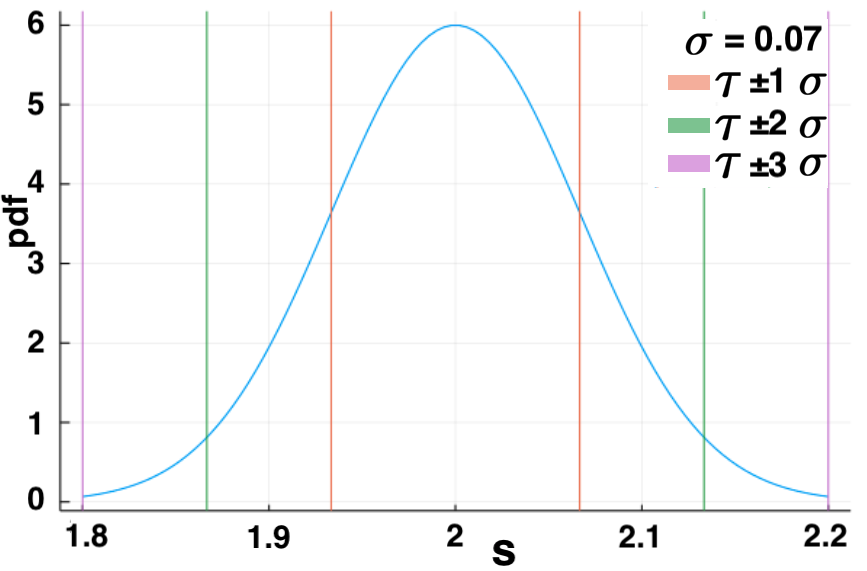
\includegraphics[width=7cm,height=5cm]{t2sig2.png}
        \caption{Truncated Gaussian distribution following $\mathcal{N}(2,(\sigma_{max}\times0.1)^2)$}
        \label{}
    \end{subfigure}
    \caption{PDF of truncated Gaussian distribution with mean $\tau=2$ and integration domain $[2-3\sigma,2+3\sigma]$.}
    \label{fig:pdf2}
\end{figure}
We see that $\sigma$ is responsible for scaling on the $x$-axis, while the truncation constant $\Phi_c$ scales the $y$-axis, ensuring the pdf integrates to $1$ across the integration domain. For the implementation of the quadrature rule, the number of sub-intervals $N$ was chosen to be $N=50$. The consideration for such a choice involves both quadrature accuracy and computational efficiency. The motivation for setting $N=50$ was dependant on evaluating `test' integrals and simulation `test' DDEs, for which the results are presented in the remainder of this section.

\section{Linear Analysis}\label{section:distlin}
The system of equations is given by
\begin{equation}\label{dist}
  \begin{split}
  \frac{\partial u}{\partial t}&=D_u\frac{\partial^2u}{\partial x^2}+a-u-2u^2v+3\int_a^bk(s)\hat{u}^2\hat{v} \text{ds}\\
  \frac{\partial v}{\partial t}&=D_v\frac{\partial^2v}{\partial x^2}+b-u^2v,
\end{split}
\end{equation}
where $u=u(x,t)$, $v=v(x,t)$, $\hat{u}=u(x,t-s)$ and $\hat{v}=v(x,t-s)$. $k(s)$ is the truncated Gaussian distribution, integrating to $1$ between constant limits $a$ and $b$, and is given by
\begin{equation}
k(s)=\frac{\Phi_c}{\sqrt{2\pi}\sigma}\exp\left(-\frac{1}{2}\left(\frac{s-\tau}{\sigma}\right)^2\right),
\end{equation}
for some mean $\tau$ and standard deviation $\sigma$. $\Phi_c$ denotes the truncation scaling factor. Denoting the steady-state $(u_\star,v_\star)$, and taking a small perturbation about the steady-state $u=u_\star+\delta\xi$, $v=v_\star+\delta\eta$, where $|\delta|\ll1$, we can write the equation for $u$ in \eqref{dist} as

\begin{equation}\label{perturb}
  \delta\frac{\partial \xi}{\partial t}=\delta D_u\frac{\partial^2\xi}{\partial x^2}+f(u_\star+\delta\xi, v_\star+\delta\eta)+g(u_\star+\delta\hat{\xi},v_\star+\delta\hat{\eta}) ,
\end{equation}
where $f(u,v)=a-u+2u^2v$ and $g(\hat{u},\hat{v})=3\int_a^bk(s)\hat{u}^2\hat{v} \text{ds}$. The $\hat{\xi}$ notation is used to denote the perturbation evaluated at a delay $\hat{\xi}=\xi(x,t-s)$. Taylor expanding equation \eqref{perturb} for the $f$ term about the steady-state and evaluating the $g$ term, up to $O(\epsilon)$, yields

\begin{dmath}\label{taylor}
  \delta\frac{\partial \xi}{\partial t}=\delta D_u\frac{\partial^2\xi}{\partial x^2}+f(u_\star,v_\star)+3u_\star^2v_\star\int_a^bk(s)\text{ds}+\delta\left[\xi f_u(u_\star,v_\star)+\eta f_v(u_\star,v_\star)+6u_\star v_\star\int_a^bk(s)\hat{\xi}\text{ds}+3u_\star^2\int_a^bk(s)\hat{\eta}\text{ds}
  \right].
\end{dmath}
We use the notation $f_u$ to denote the derivative of function $f$ with respect $u$. Using the facts that the truncated Guassian $k(s)$ integrates to $1$ over $[a,b]$, and evaluation the expressions $f_u(u_\star,v_\star)$ and $f_v(u_\star,v_\star)$, equation \eqref{taylor} can be simplified to

\begin{equation}\label{linu}
  \delta \frac{\partial \xi}{\partial t}=\delta D_u\frac{\partial^2\xi}{\partial x^2}+\delta\left[\xi(-1-4u_\star v_\star)-2\eta u_\star^2 +6u_\star v_\star\int_a^bk(s)\hat{\xi}\text{ds}+3u_\star^2\int_a^bk(s)\hat{\eta}\text{ds}\right].
\end{equation}
The linearised dynmacs for $v$ are more simply given by
\begin{equation}\label{linv}
\delta \frac{\partial\eta}{\partial t}=\delta D_v\frac{\partial^2\eta}{\partial x^2}-\delta\left[2\xi u_\star v_\star+\eta u_\star^2\right].
\end{equation}
Dividing through by $\delta$ and substituting in an ansatz of the form $\xi=\xi_0e^{\lambda t}\cos(k\pi x)$ \cite{yigaffneyli} into \eqref{linu} and $\eta=\eta_0e^{\lambda t}\cos(k\pi x)$ into \eqref{linv}, and then dividing through by $e^{\lambda t}$ and $\cos(k\pi x)$, results in

\begin{equation}\label{sysof}
  \begin{split}
\lambda\xi_0&=-D_uk^2\pi^2\xi_0+\xi_0(-1-4u_\star v_\star)-2\eta_0u_\star^2+6\xi_0u_\star v_\star E+3\xi_0u_\star^2E \\
\lambda\eta_0&=-D_vk^2\pi^2\eta_0-2\xi_0u_\star v_\star-\eta_0u_\star^2,
\end{split}
\end{equation}
where $E=\int_a^bk(s)e^{-\lambda s}\text{ds}$. We can write equation \eqref{sysof} as a homogeneous linear system for $(\xi_0,\eta_0)^T$, given by

\begin{equation}
\underbrace{\begin{pmatrix}-1-4u_\star v_\star-D_uk^2\pi^2+6u_\star v_\star E-\lambda&-2u_\star^2+3u_\star^2E\\-2u_\star v_\star&-u_\star^2-D_vk^2\pi^2-\lambda \end{pmatrix}}_{\textbf{M}}\begin{pmatrix}\xi_0\\\eta_0\end{pmatrix}=\begin{pmatrix}0\\0\end{pmatrix}.
\end{equation}
Looking for non-trivial solutions, we look for roots of the characteristic equation, namely $D_k=\text{det}(\textbf{M})=0$. The characteristic equation, $D_k$, is given as
\begin{equation}\label{characdist}
  D_k=\lambda^2+\alpha_k\lambda+\beta_k+(\gamma_k\lambda+\delta_k)E=0,
\end{equation}
where
\begin{align}
\alpha_k&=(D_u+D_v)k^2\pi^2+u_\star^2+4u_\star v_\star+1\\
\beta_k&=(D_v\pi^2k^2+u_\star^2)(D_u\pi^2k^2+4u_\star v_\star+1)-4u_\star^3v_\star\\
\gamma_k&=-6u_\star v_\star\\
\delta_k&=-6D_vu_\star v_\star k^2\pi^2.
\end{align}

Finally, we note that the expression $E$ can be evaluated as
\begin{equation}
E=\int_a^bk(s)e^{-\lambda s}ds=\frac{\Phi_c}{2}\left[\exp\left(\frac{\lambda(\lambda\sigma^2-2\tau)}{2}\right) \text{erf} \left(\frac{\lambda\sigma^2+s-\tau}{\sqrt{2}\sigma}\right)\right]\Bigg|_a^b.
\end{equation}
The charactersitic equation \eqref{characdist} cannot trivially be split into it's real and imaginary components due to the error function term in $E$ as was done in the fixed delay case. We therefore cannot explicitly compute the stability lines in $(a,b)$ parameter space. We can however range over $(a,b)$ and compute $\max_k(\Re(\lambda_k))$ for different $\tau$, and produce plots similar to those in figures \ref{fig:dispfixed} and \ref{fig:lambdavary}. We use these plots to pseudo-analytically prove that, using a symmetric Gaussian distribution centred at mean $\tau$ will not change the time-to pattern seen for a fixed delay of $\tau$, independent of the standard deviation of the distribution $\sigma$. We first plot $\max_k(\Re(\lambda_k))$ against $\tau$, as seen analogously in figure \ref{fig:dispfixed} for the fixed delay case, for multiple parameters $(a,b,\tau,\sigma)$, and compares these to the fixed delay case. Since physically we cannot have negative delays, we require the lower integration limit to be positive. Namely, for a given mean $\tau$, we require $\tau-3\sigma>0$. We therefore define a maximum $\sigma$ value by $\sigma_{max}=\tau / 3$. By ensuring $\sigma<\sigma_{max}$, we ensure only positive delays are considered. Figures \ref{fig:p1}, \ref{fig:p2}, and \ref{fig:p3} show $\max_k(\Re(\lambda_k))$ plotted against $\tau\in[0,1]$ for three different parameter sets $(a,b)=\{(0.3,1.2), (0.1,0.9), (0.4,0.4)\}$. For each parameter set, plots are produced with different $\sigma$ values as a fraction of $\sigma_{max}$, as well as for the fixed delay case. We note that in the distributed delay case, as we vary $\tau$, $\sigma_{max}$ and thus the integration limits both change as functions of $\tau$. The diffusive coefficients were set as $D_u=\epsilon^2/L^2$, $D_v=1/L^2$,  with  $\epsilon^2=0.001$, $L=30\sqrt{0.05}$, and $k$ varied from $[0,50]$ at regular discrete intervals of $1$.

% PARAMTER SET 1
\begin{figure}[H]
    \centering
    \begin{subfigure}[b]{0.45\textwidth}
        \centering
        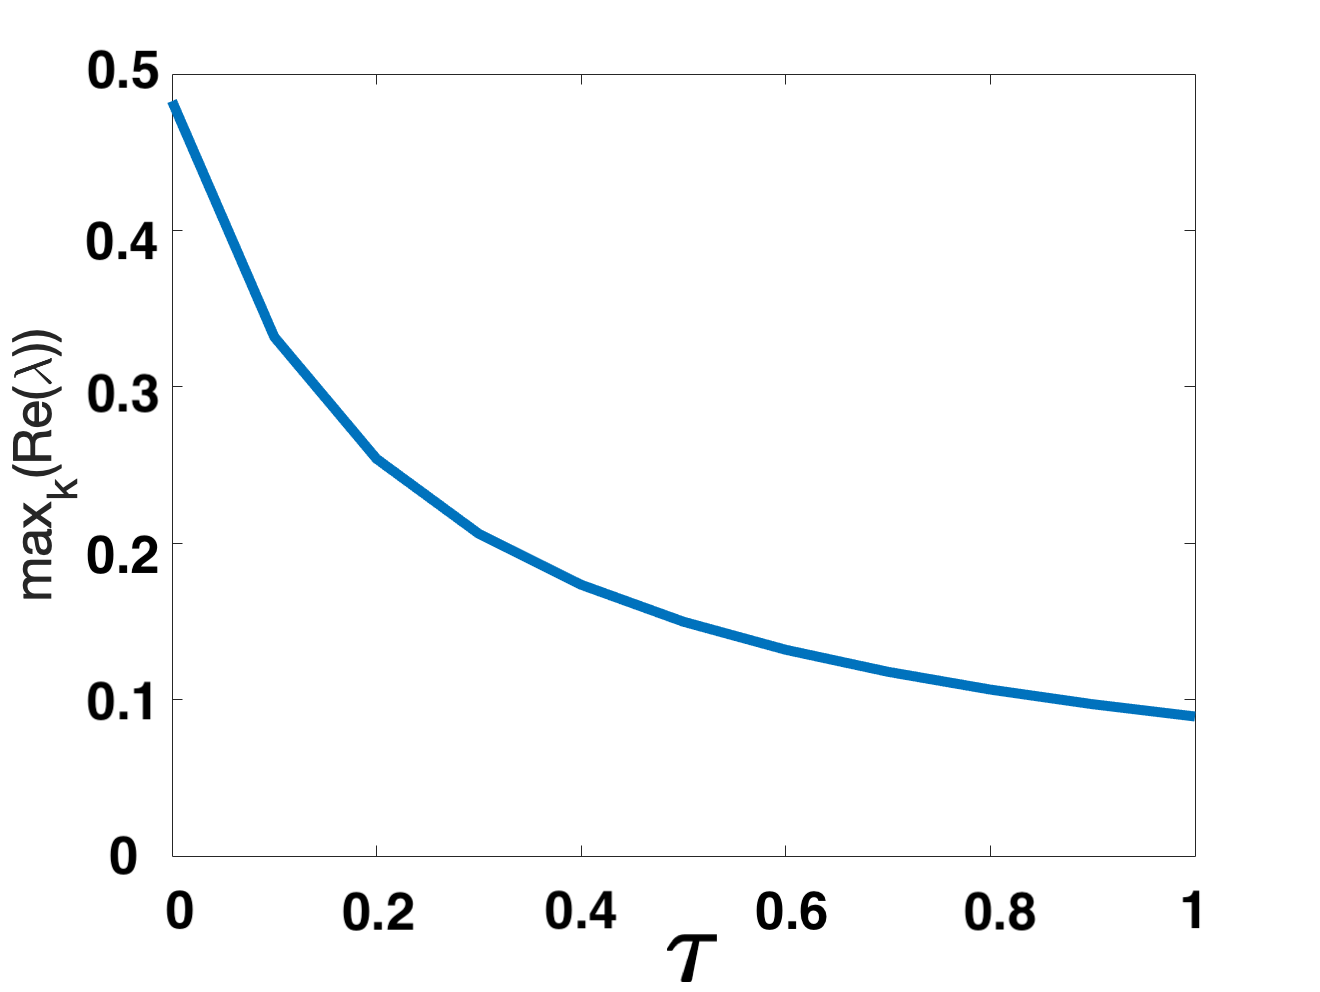
\includegraphics[width=7cm,height=5cm]{p1fixed.png}
        \caption{Fixed delay case.}
        \label{}
    \end{subfigure}
    \hfill
    \begin{subfigure}[b]{0.45\textwidth}
        \centering
        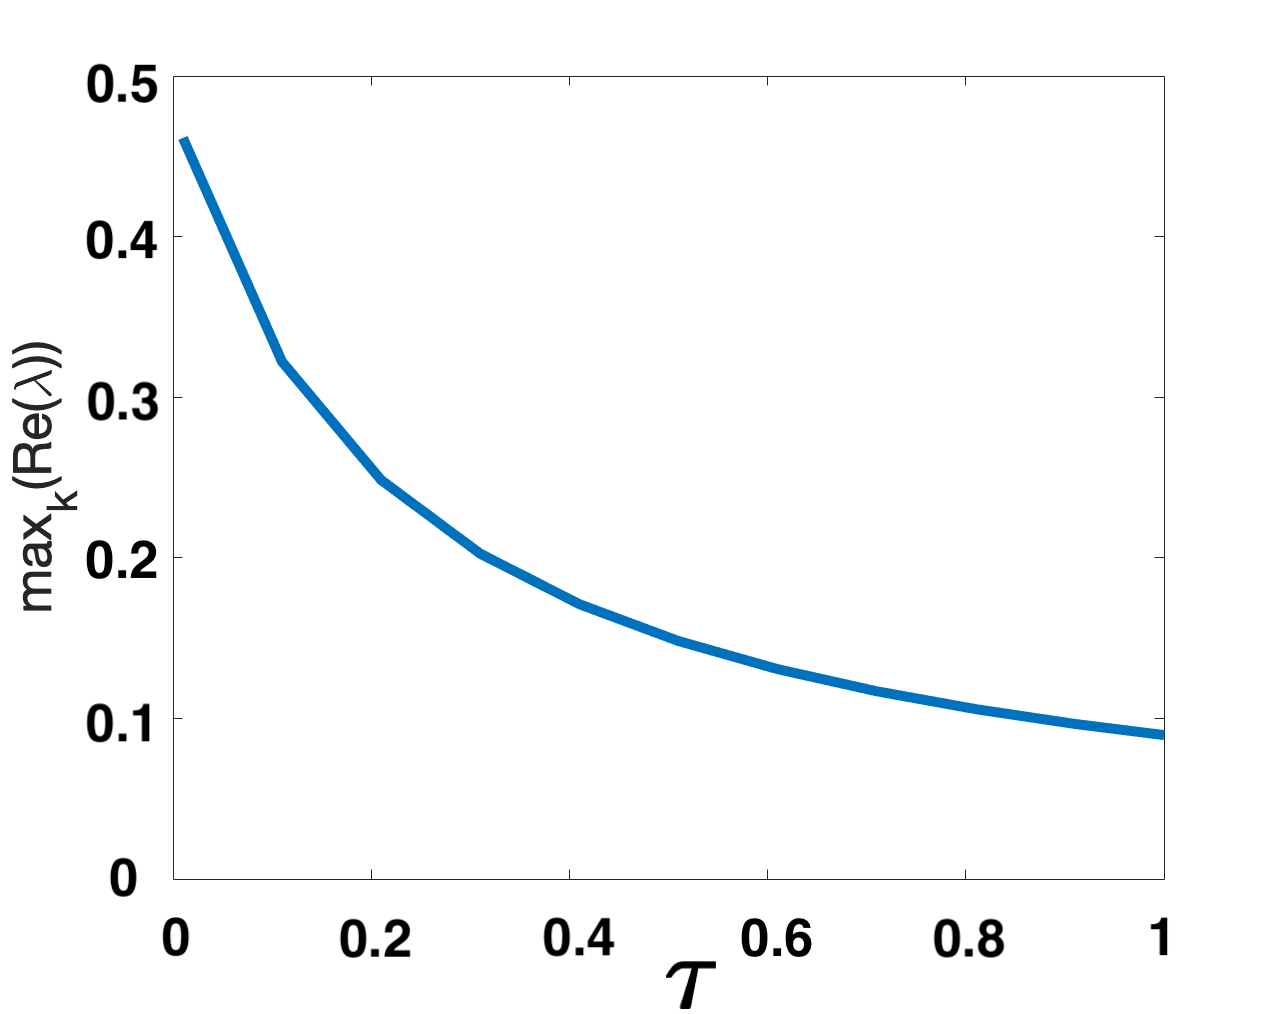
\includegraphics[width=7cm,height=5cm]{p1sigmax.png}
        \caption{Distributed delay with $\sigma=\sigma_{max}\times0.99$.}
        \label{}
    \end{subfigure}
    \hfill
    \begin{subfigure}[b]{0.45\textwidth}
        \centering
        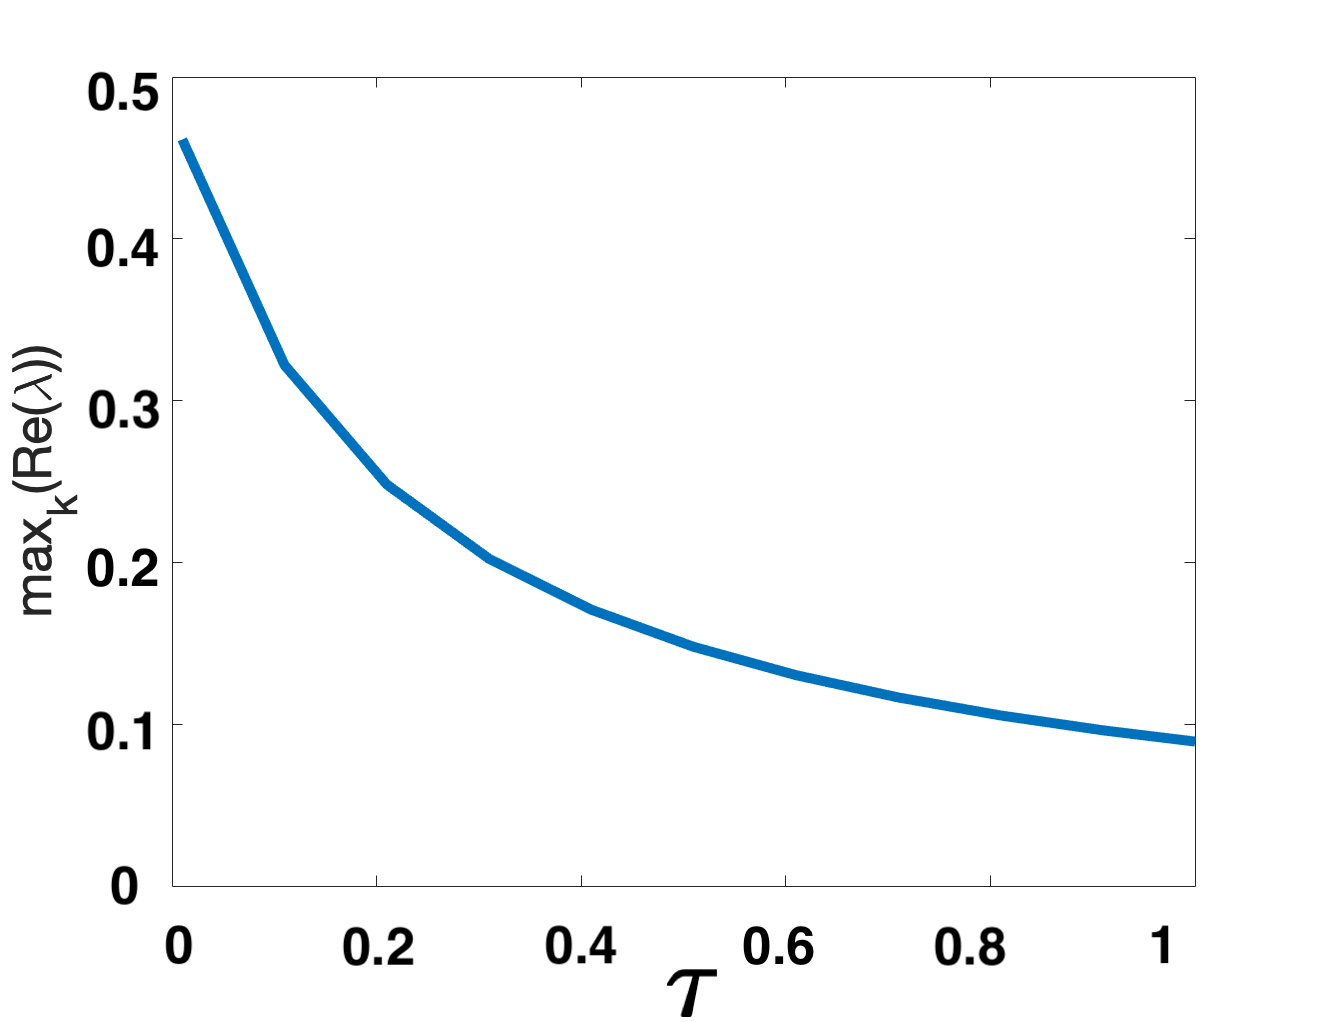
\includegraphics[width=7cm,height=5cm]{p1sigmax5.png}
        \caption{Distributed delay with $\sigma=\sigma_{max}\times0.2$.}
        \label{}
    \end{subfigure}
    \hfill
    \begin{subfigure}[b]{0.45\textwidth}
        \centering
        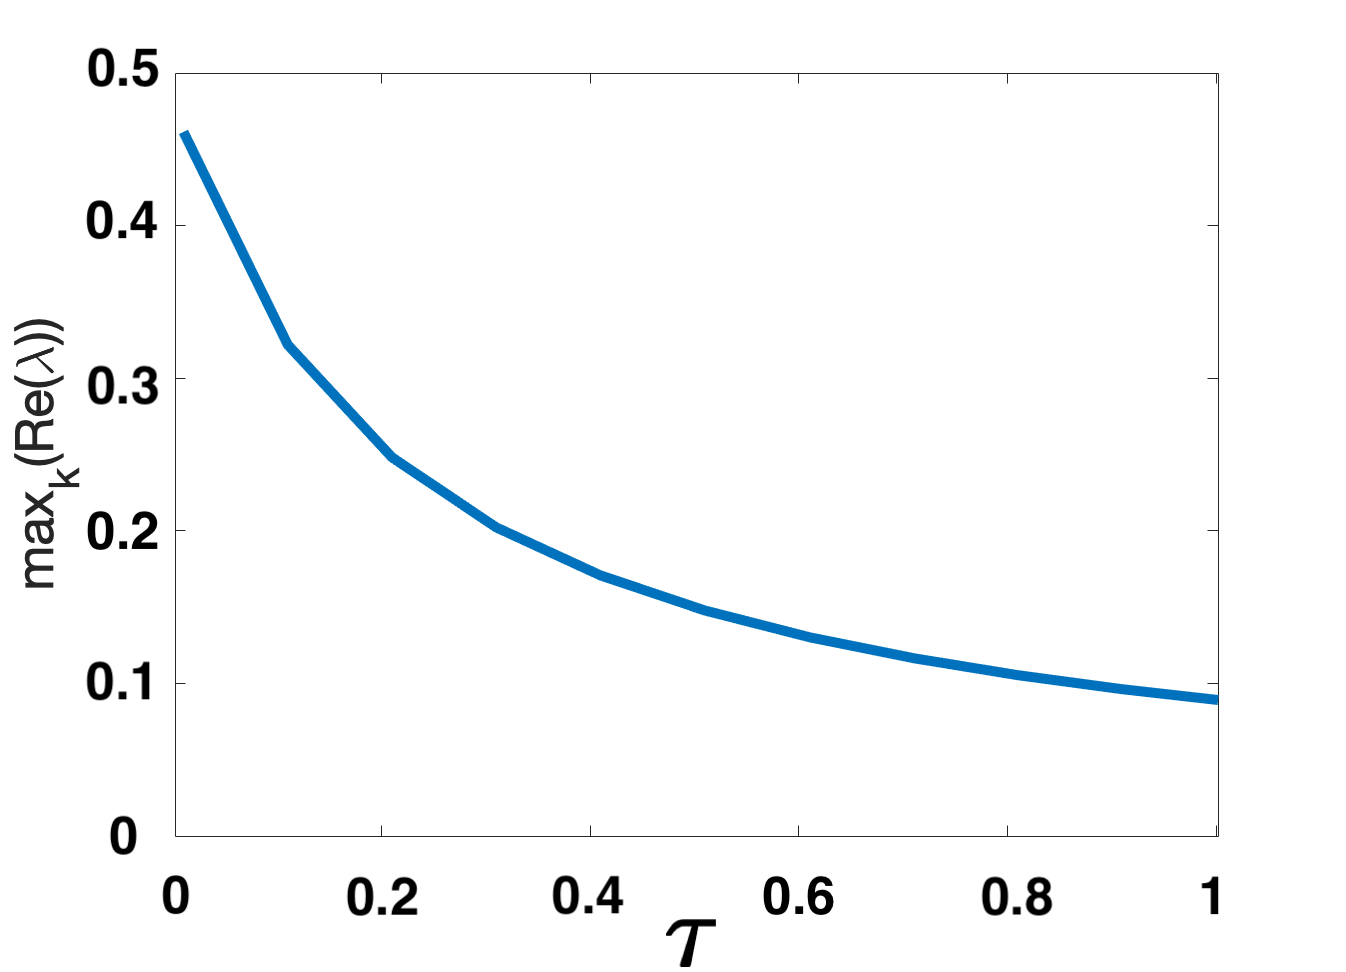
\includegraphics[width=7cm,height=5cm]{p1sigmax10.png}
        \caption{Distributed delay with $\sigma=\sigma_{max}\times0.1$.}
        \label{}
    \end{subfigure}
    \caption{$\max_k(\Re(\lambda_k))$ plotted against $\tau\in[0,1]$ for parameter set $(a,b,\epsilon^2)=(0.3,1.2,0.001)$. $L=30\sqrt{0.05}$ and $k$ varied over $[0,50]$ at regular discrete intervals of $1$.}
    \label{fig:p1}
\end{figure}
% PARAMTER SET 2
\begin{figure}[H]
    \centering
    \begin{subfigure}[b]{0.45\textwidth}
        \centering
        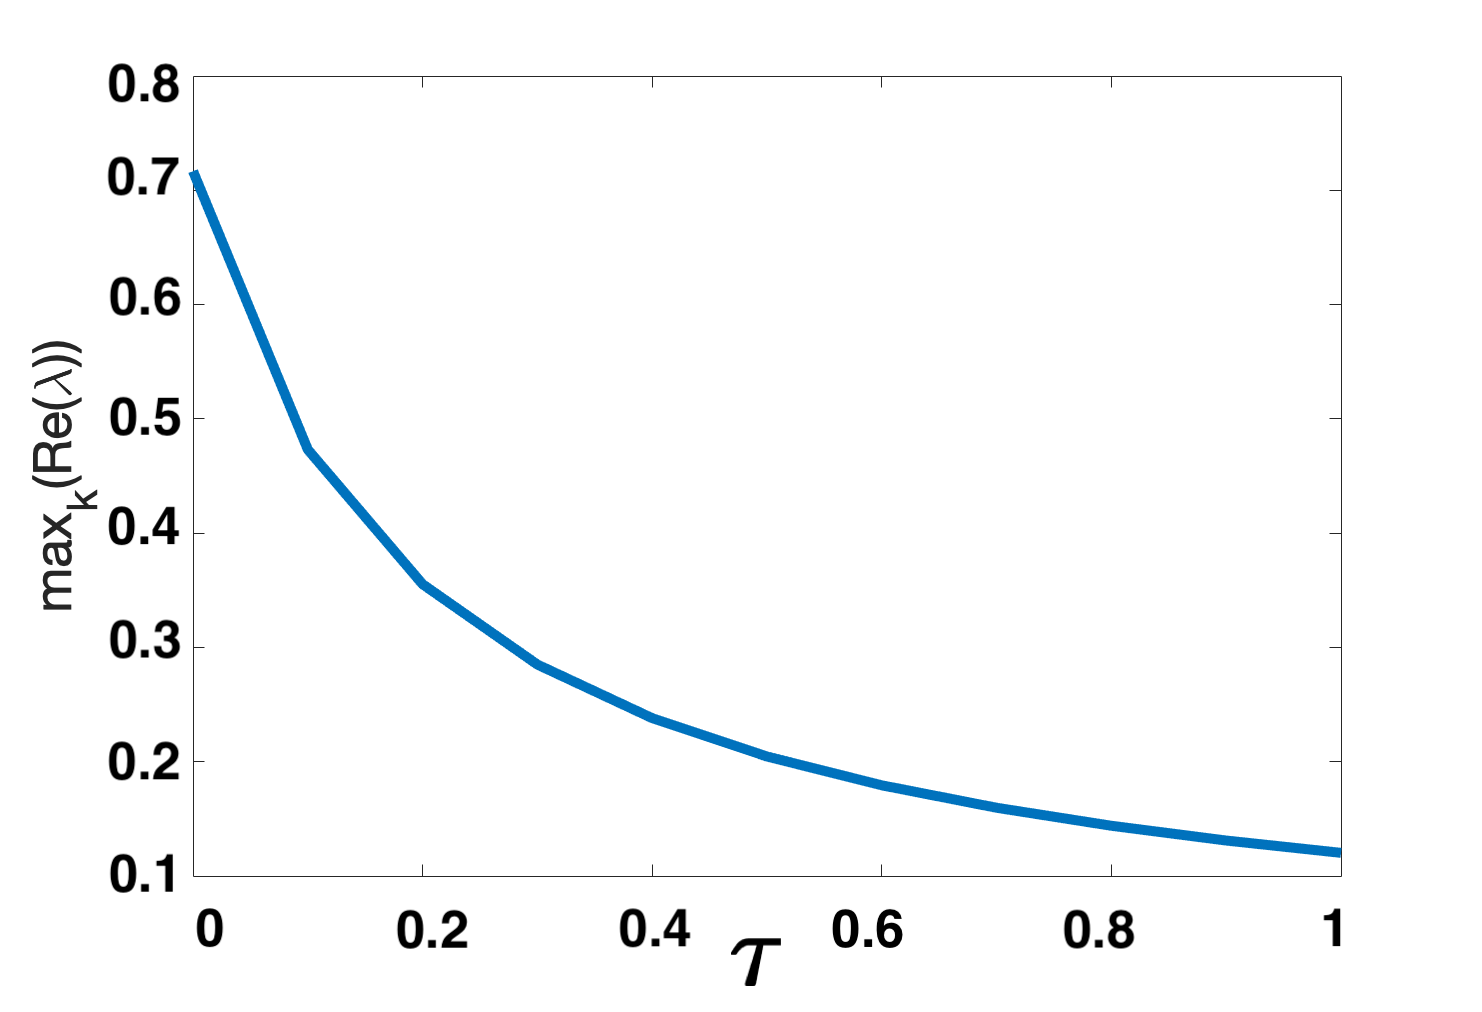
\includegraphics[width=7cm,height=5cm]{p2fixed.png}
        \caption{Fixed delay case.}
        \label{}
    \end{subfigure}
    \hfill
    \begin{subfigure}[b]{0.45\textwidth}
        \centering
        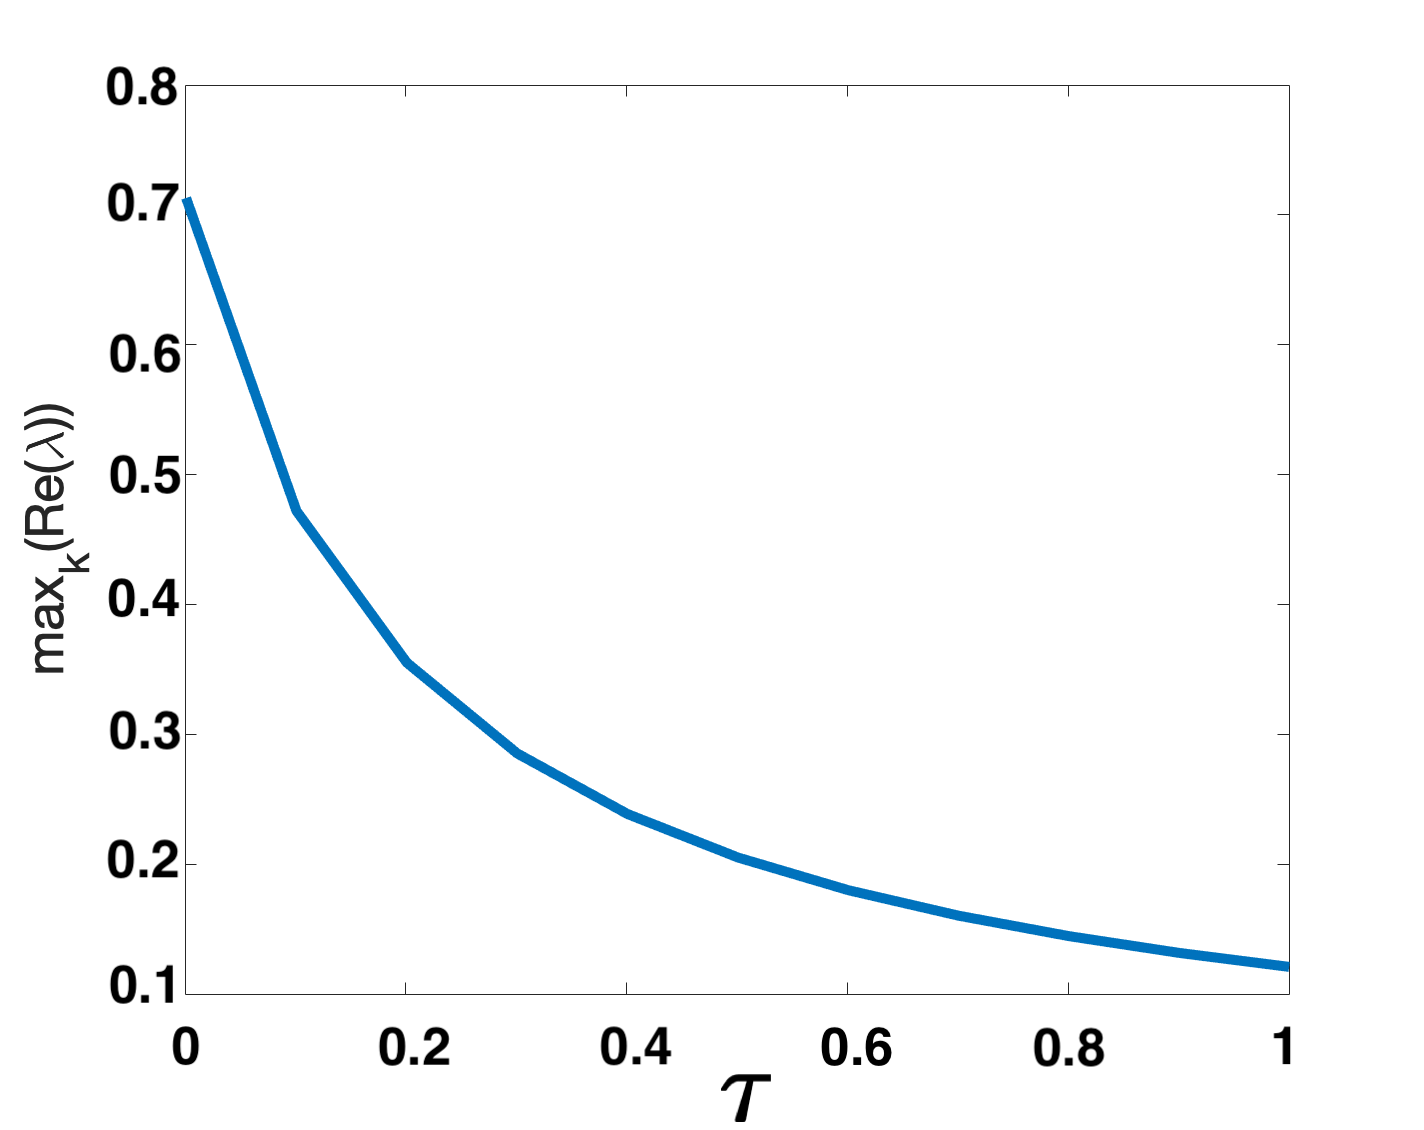
\includegraphics[width=7cm,height=5cm]{p2sigmax.png}
        \caption{Distributed delay with $\sigma=\sigma_{max}\times0.99$.}
        \label{}
    \end{subfigure}
    \hfill
    \begin{subfigure}[b]{0.45\textwidth}
        \centering
        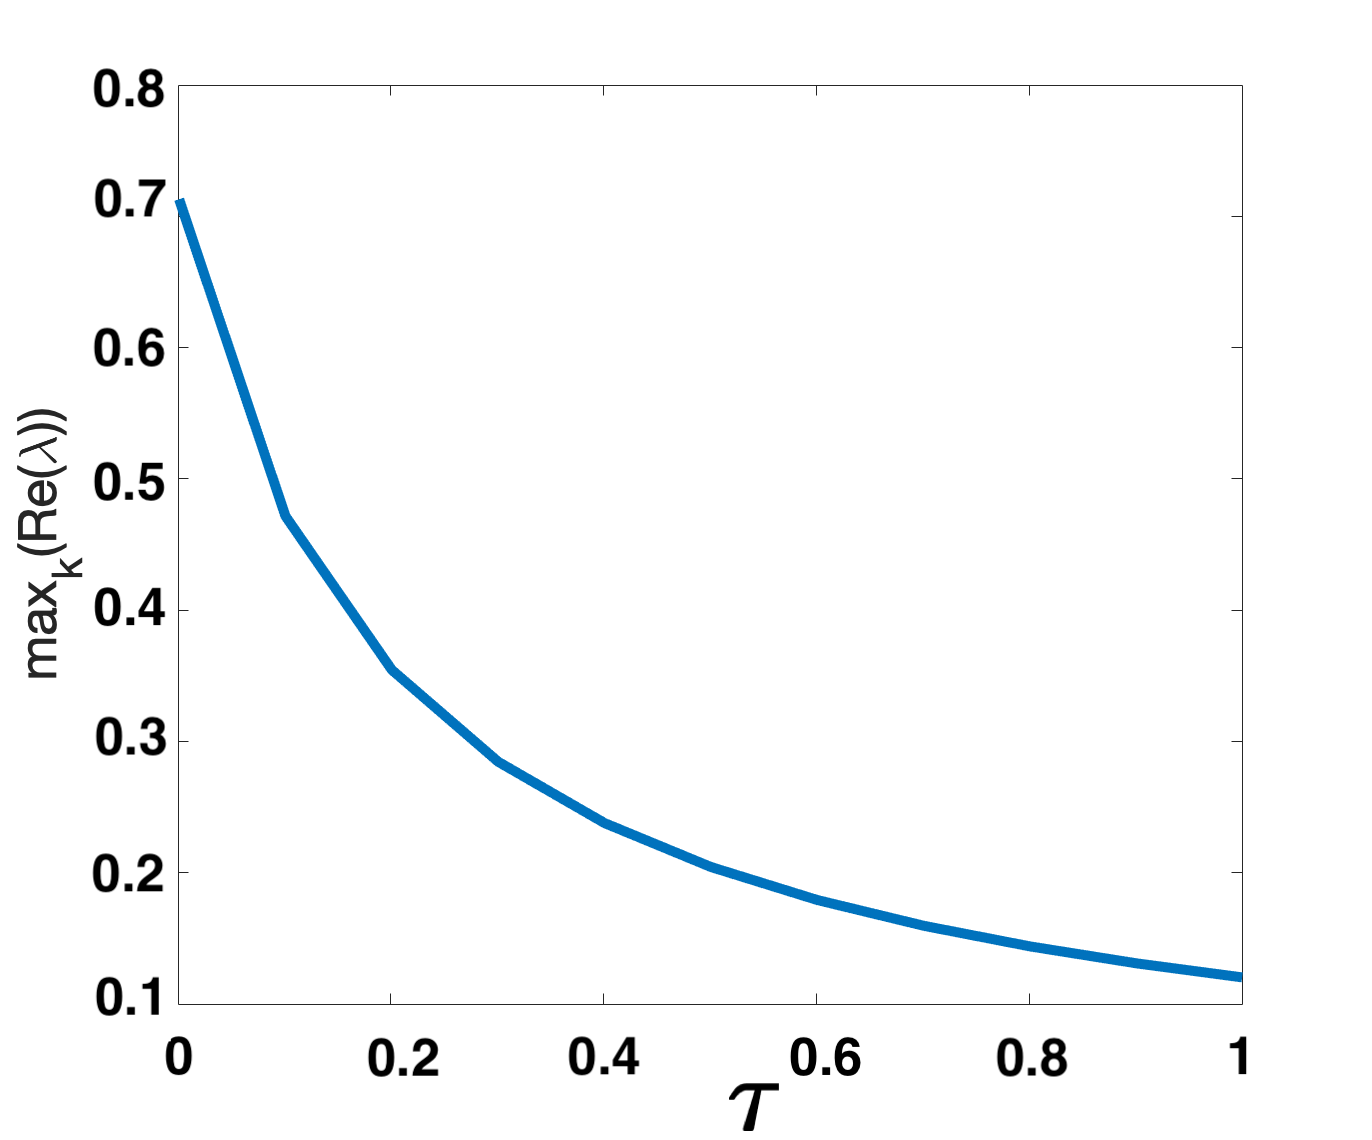
\includegraphics[width=7cm,height=5cm]{p2sigmax5.png}
        \caption{Distributed delay with $\sigma=\sigma_{max}\times0.2$.}
        \label{}
    \end{subfigure}
    \hfill
    \begin{subfigure}[b]{0.45\textwidth}
        \centering
        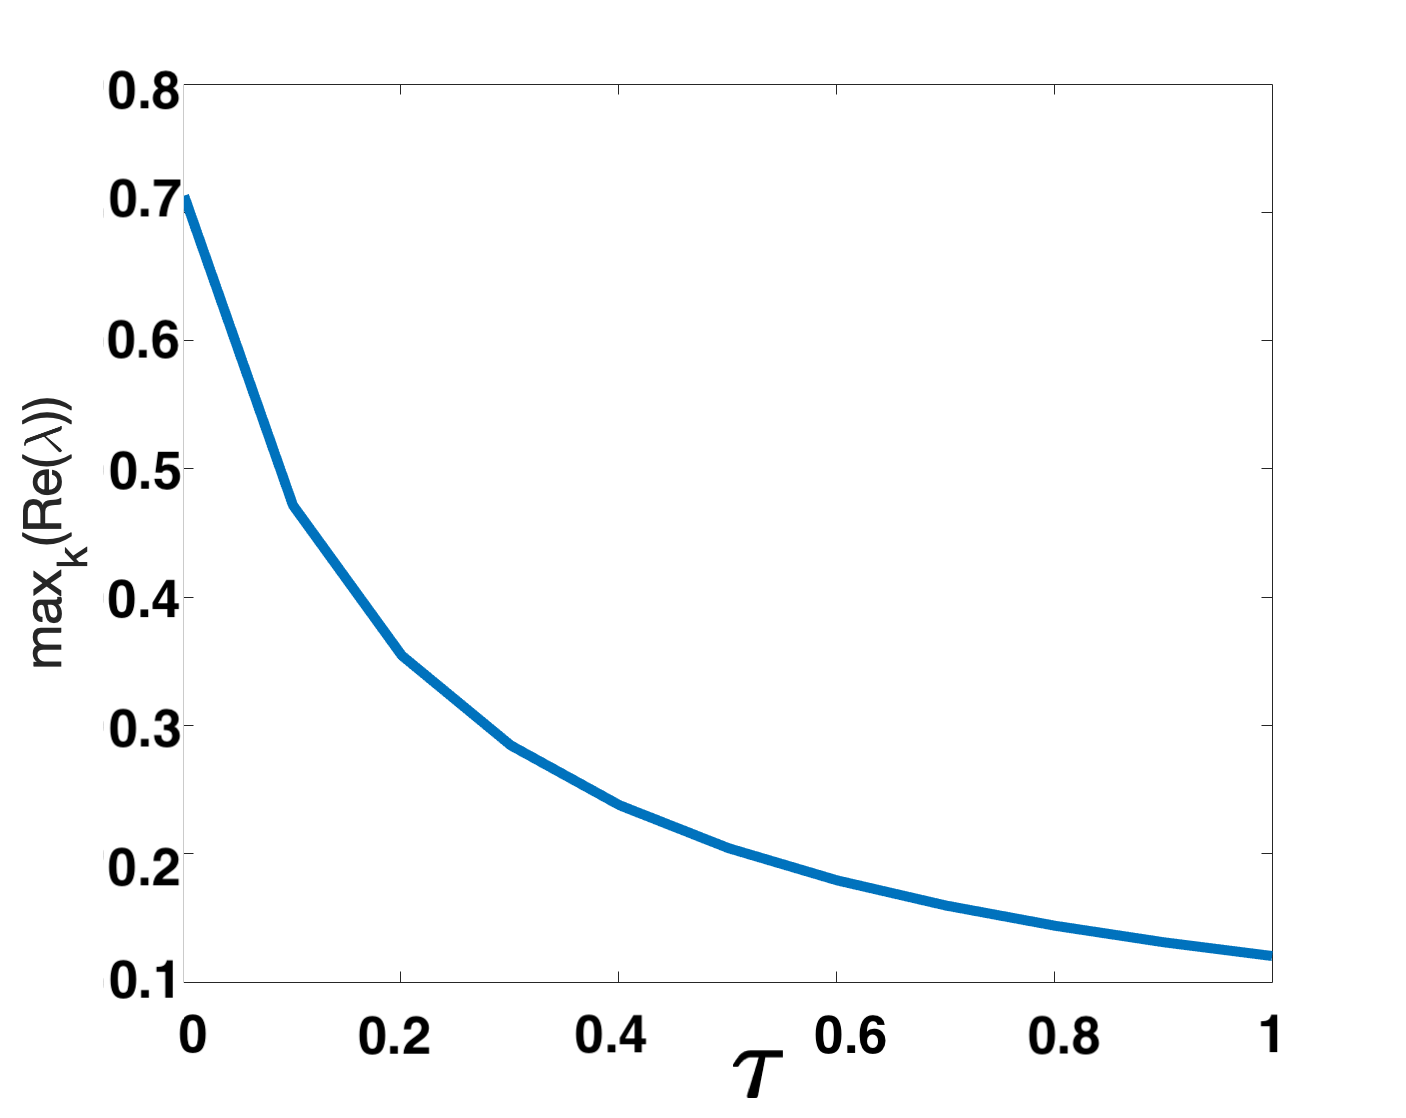
\includegraphics[width=7cm,height=5cm]{p2sigmax10.png}
        \caption{Distributed delay with $\sigma=\sigma_{max}\times0.1$.}
        \label{}
    \end{subfigure}
    \caption{$\max_k(\Re(\lambda_k))$ plotted against $\tau\in[0,1]$ for parameter set $(a,b,\epsilon^2)=(0.1,0.9,0.001)$. $L=30\sqrt{0.05}$ and $k$ varied over $[0,50]$ at regular discrete intervals of $1$.}
    \label{fig:p2}
\end{figure}
% PARAMETER SET 3
\begin{figure}[H]
    \centering
    \begin{subfigure}[b]{0.45\textwidth}
        \centering
        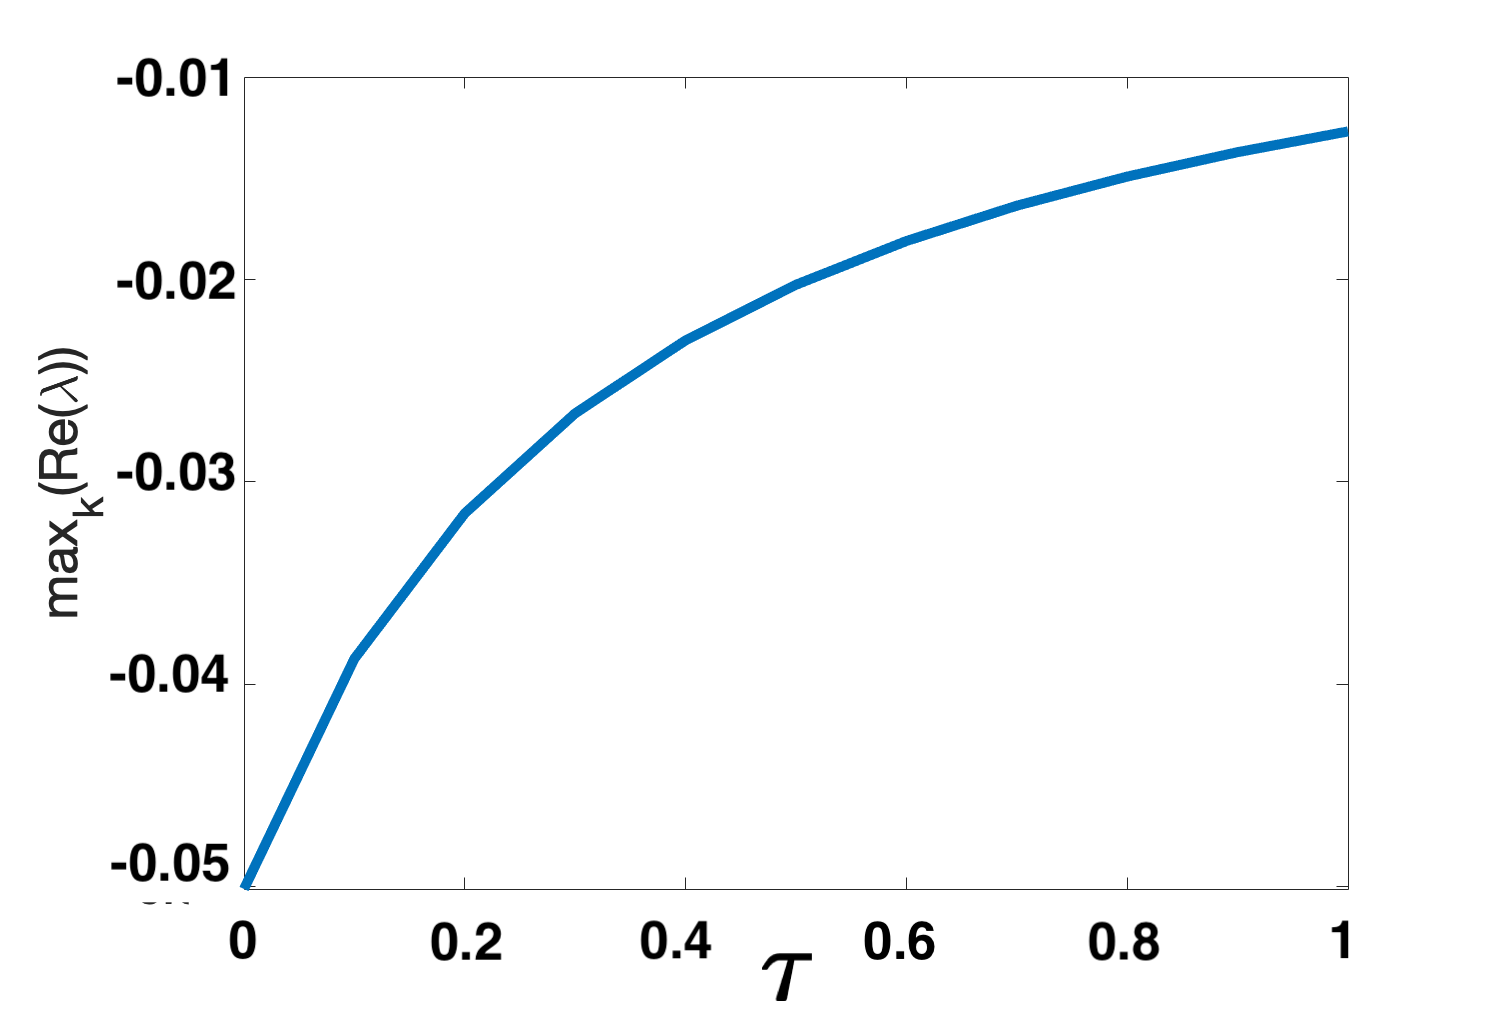
\includegraphics[width=7cm,height=5cm]{p3fixed.png}
        \caption{Fixed delay case.}
        \label{}
    \end{subfigure}
    \hfill
    \begin{subfigure}[b]{0.45\textwidth}
        \centering
        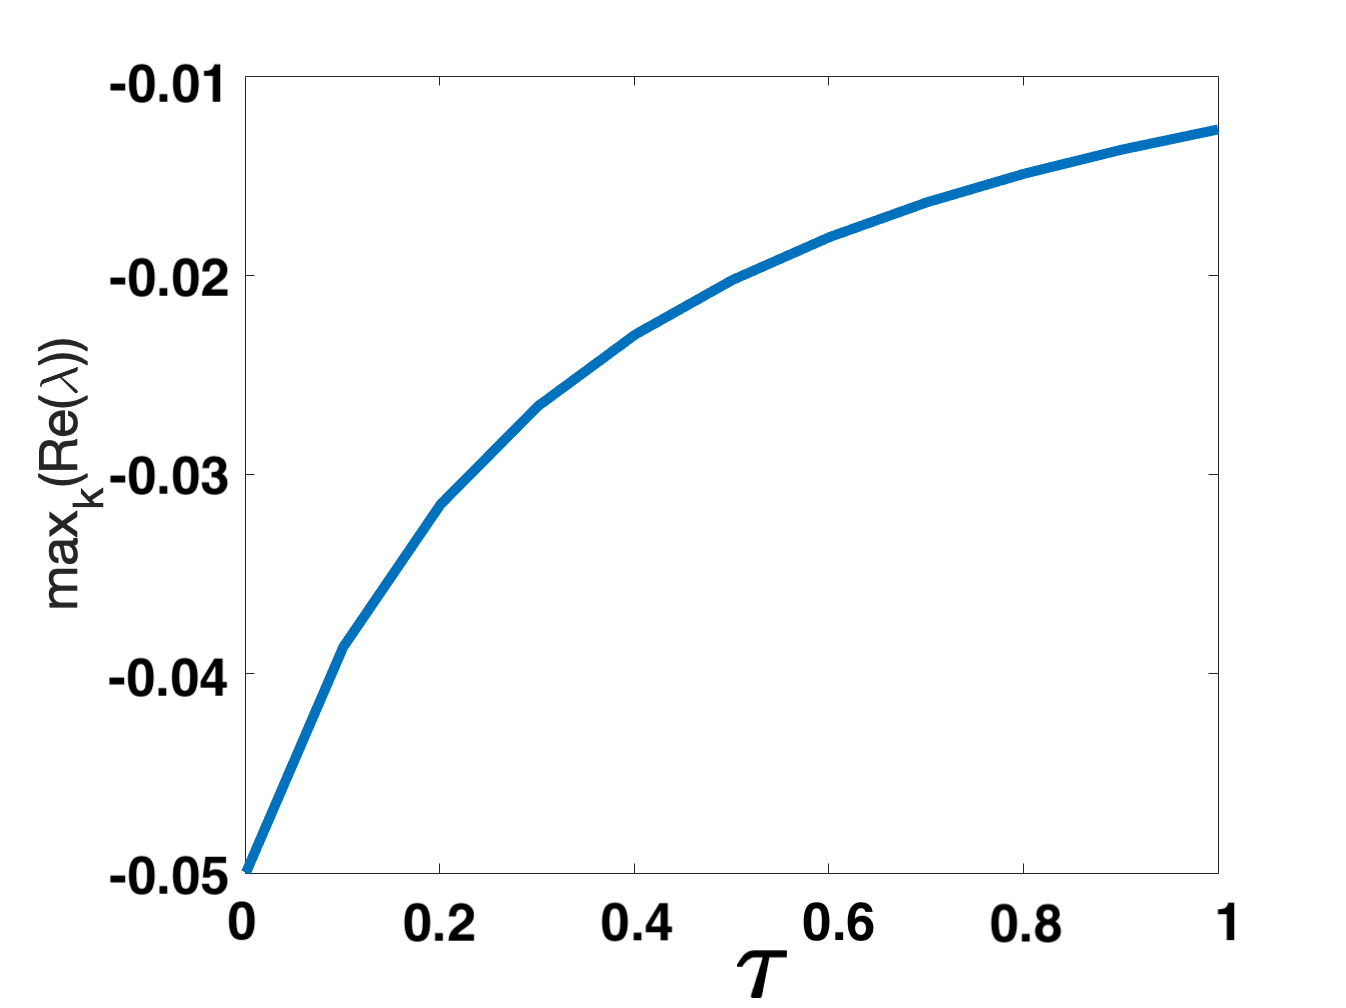
\includegraphics[width=7cm,height=5cm]{p3sigmax.png}
        \caption{Distributed delay with $\sigma=\sigma_{max}\times0.99$.}
        \label{}
    \end{subfigure}
    \hfill
    \begin{subfigure}[b]{0.45\textwidth}
        \centering
        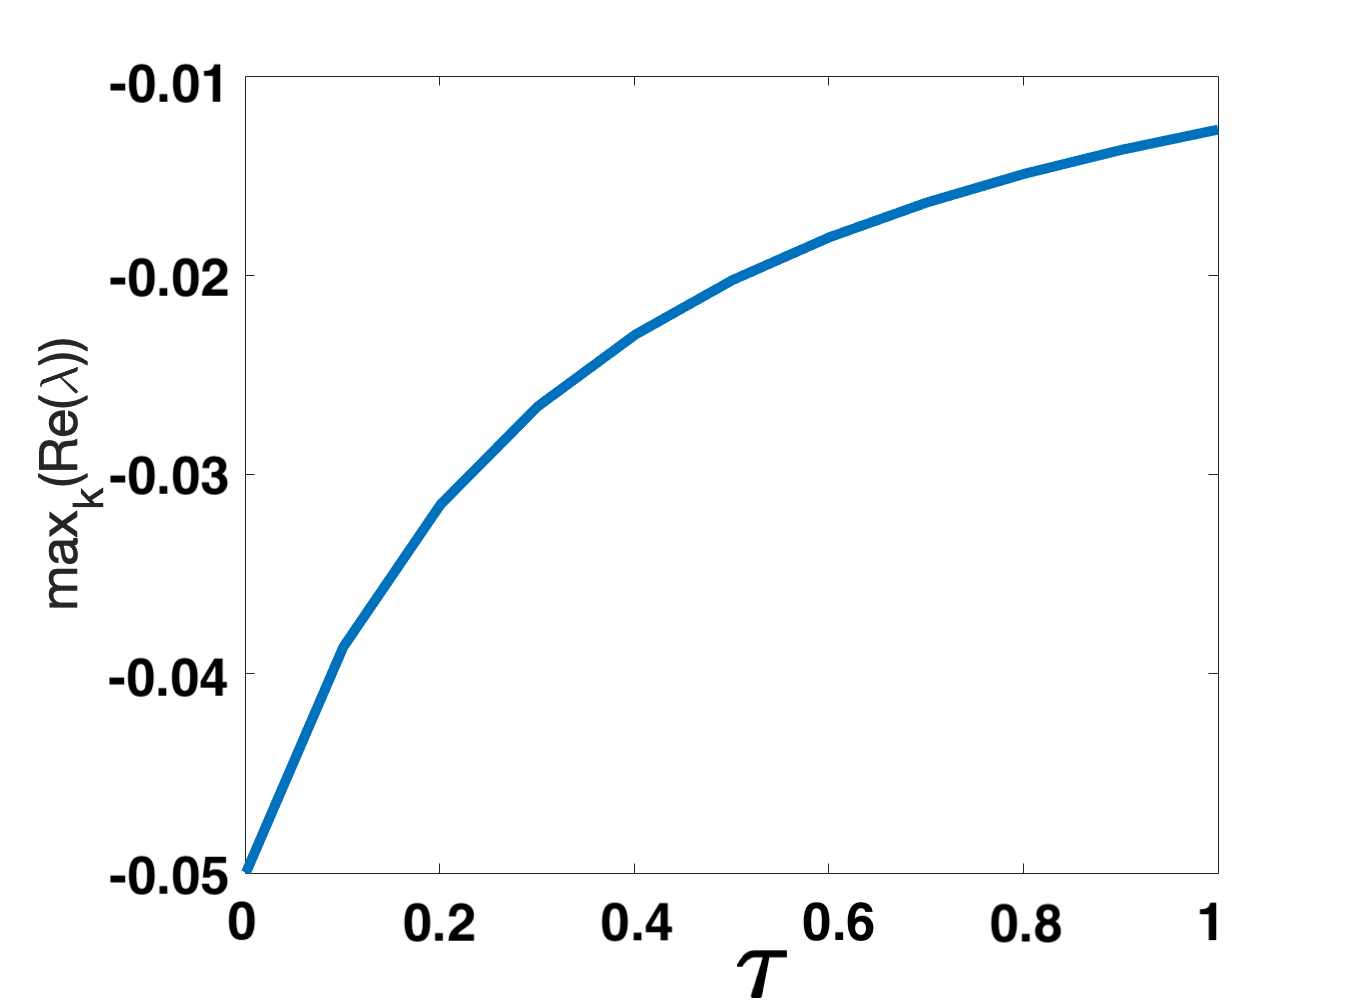
\includegraphics[width=7cm,height=5cm]{p3sigmax5.png}
        \caption{Distributed delay with $\sigma=\sigma_{max}\times0.2$.}
        \label{}
    \end{subfigure}
    \hfill
    \begin{subfigure}[b]{0.45\textwidth}
        \centering
        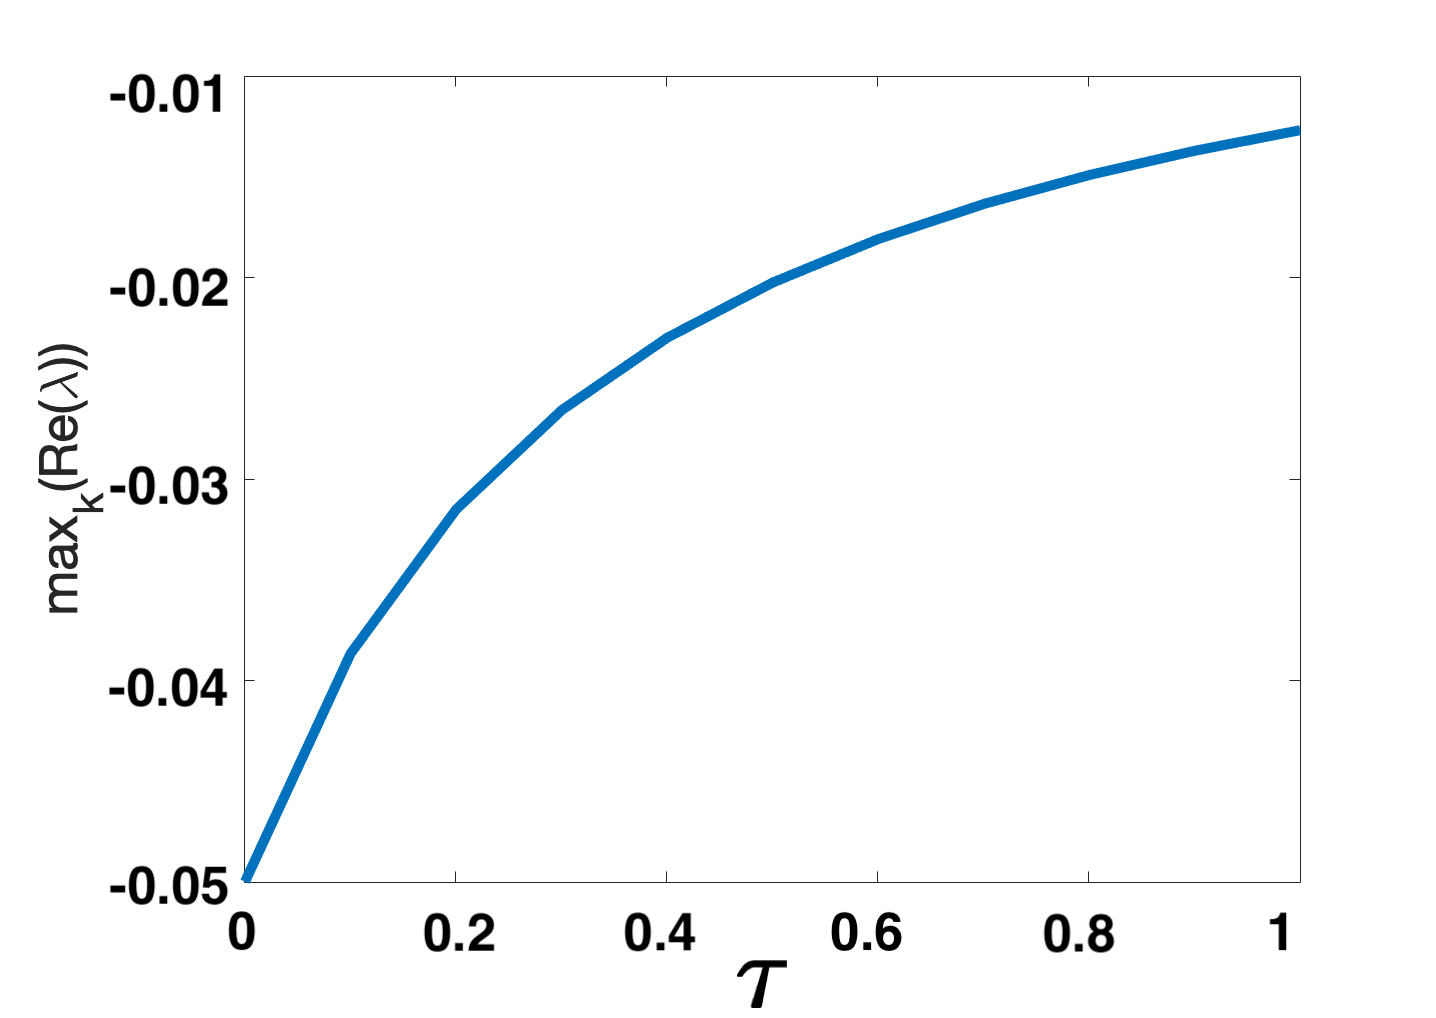
\includegraphics[width=7cm,height=5cm]{p3sigmax10.png}
        \caption{Distributed delay with $\sigma=\sigma_{max}\times0.1$.}
        \label{}
    \end{subfigure}
    \caption{$\max_k(\Re(\lambda_k))$ plotted against $\tau\in[0,1]$ for parameter set $(a,b,\epsilon^2)=(0.4,0.4,0.001)$. $L=30\sqrt{0.05}$ and $k$ varied over $[0,50]$ at regular discrete intervals of $1$.}
    \label{fig:p3}
\end{figure}

These results suggest that the time-taken to pattern formation is invariant under $\sigma$, for the parameter values chosen. The linear theory also suggests that pattern formation will occur sooner for the parameters $(a,b)=(0.1,0.9)$ than for $(a,b)=(0.3,1.2)$. This is a result we verify numerically in section \ref{section:distsim}. Here,  we plot heatmaps of $\max_k(\Re(\lambda_k))$ for varying $\sigma$ values as a fraction of $\sigma_{max}$, for $\tau\in\{0.2,1\}$. The domain length was given by $L=30\sqrt{0.05}$, and $k$ varied from $[0,50]$ at regular discrete intervals of $1$. Overlayed onto these bifurcation plots are the contour lines at $\max_k(\Re(\lambda_k))=0$ and $\Re(\lambda_0)=0$, to highlight the Turing instability region. For each $\tau$ and $\sigma$, the bifrucation plots were computed with two different $\epsilon^2$ values, $\epsilon^2=0.001,0.1$. Figures \ref{fig:distbif1} and \ref{fig:distbif3} show the results for a fixed $\tau=0.2$ with varying $\sigma$, and an $\epsilon^2=0.001,0.1$. Figures \ref{fig:distbif2} and \ref{fig:distbif4} show the analogous plots but with a fixed $\tau=1$.

\begin{figure}[H]
    \centering
    \begin{subfigure}[b]{0.45\textwidth}
        \centering
        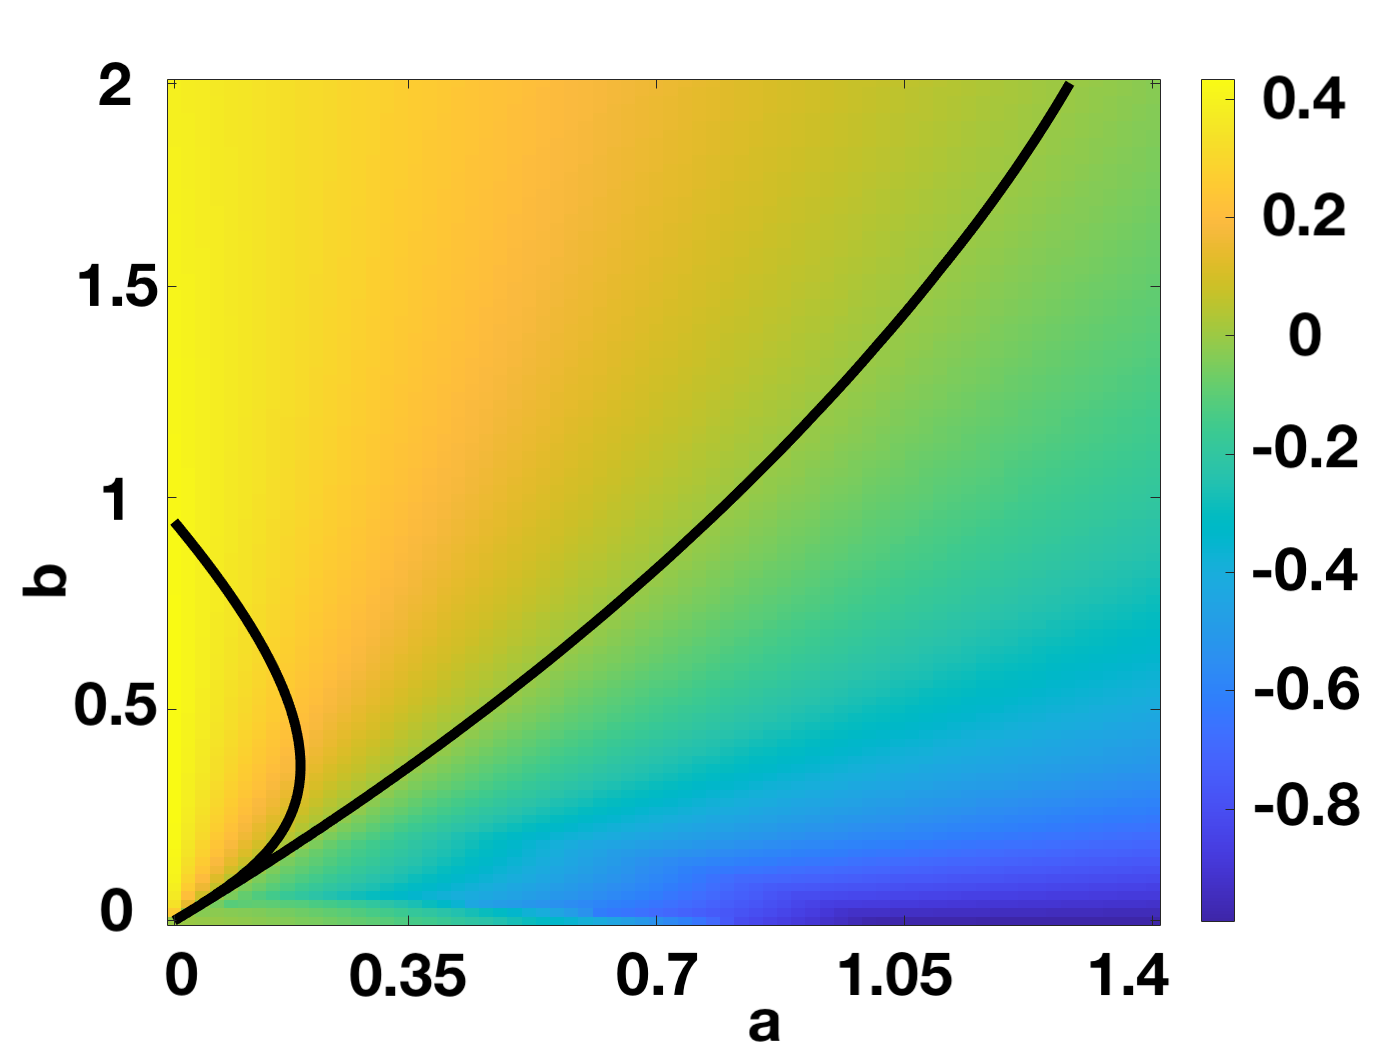
\includegraphics[width=7cm,height=4.75cm]{t1f1.png}
        \caption{Fixed delay case.}
        \label{}
    \end{subfigure}
    \hfill
    \begin{subfigure}[b]{0.45\textwidth}
        \centering
        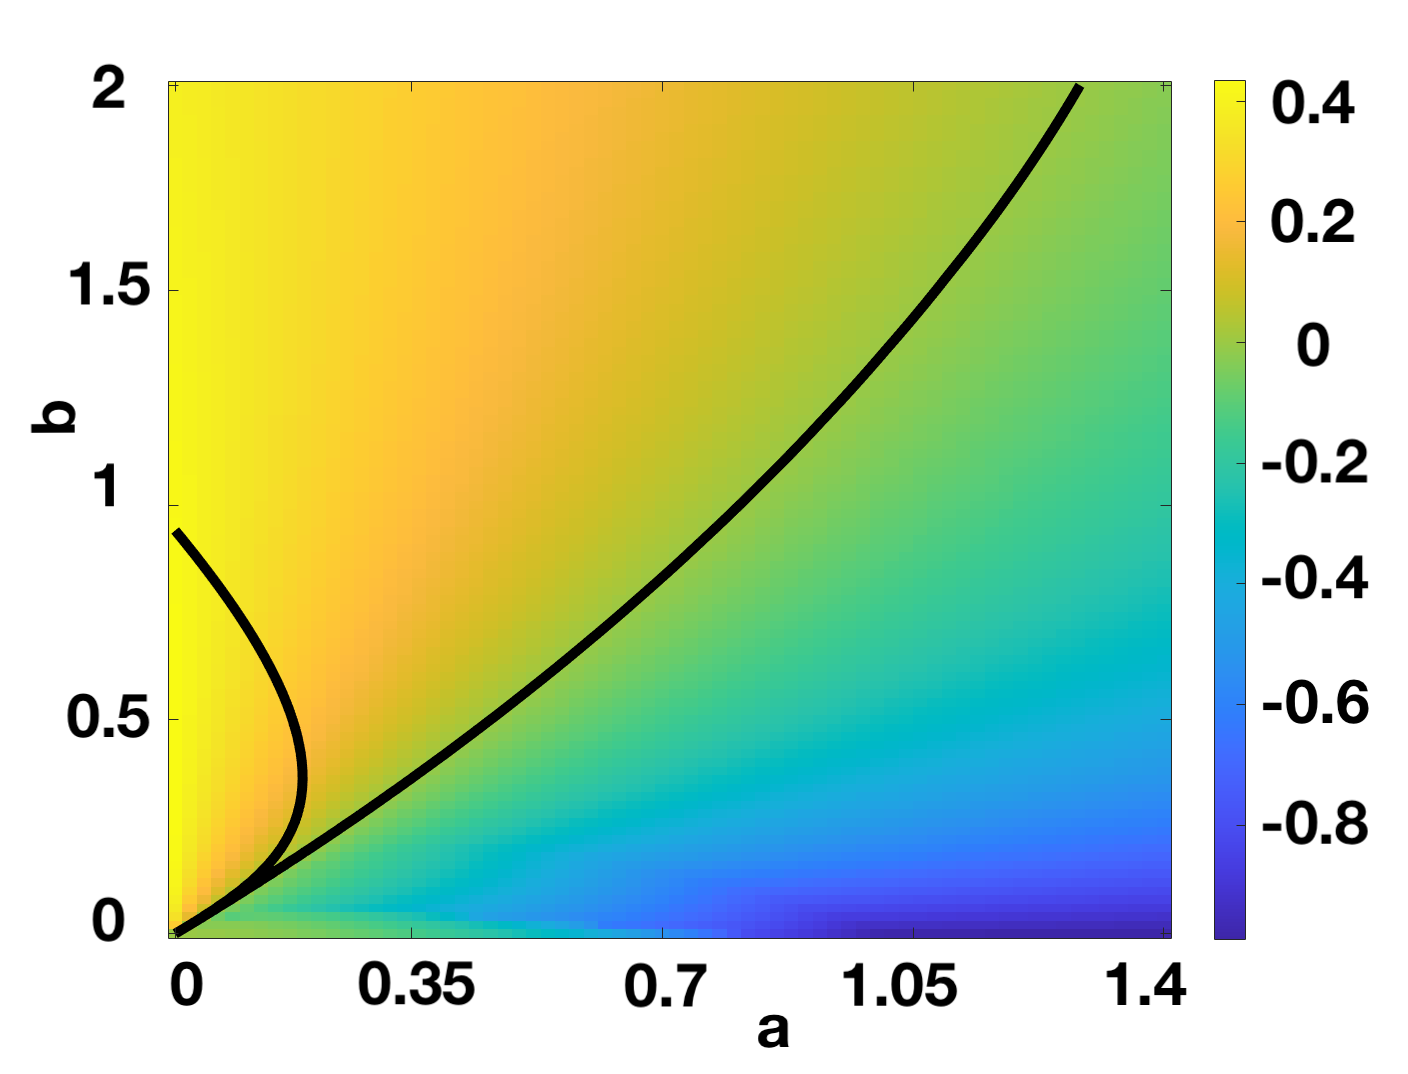
\includegraphics[width=7cm,height=4.75cm]{t1f2.png}
        \caption{Distributed delay with $\sigma=\sigma_{max}\times0.99$.}
        \label{}
    \end{subfigure}
    \hfill
    \begin{subfigure}[b]{0.45\textwidth}
        \centering
        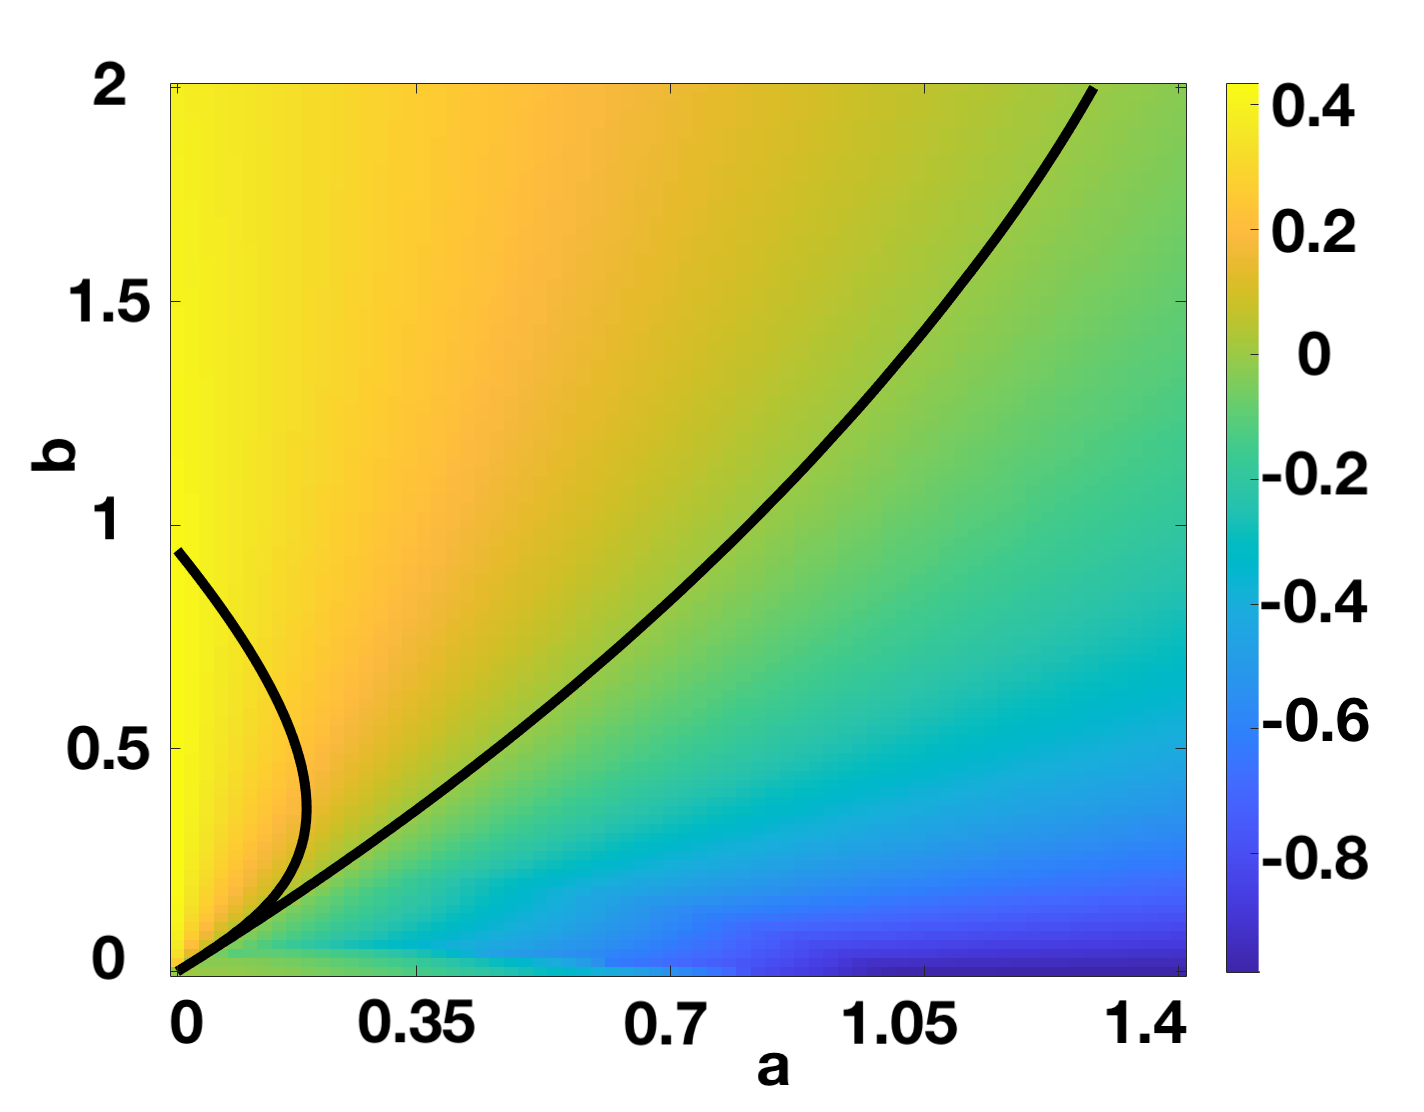
\includegraphics[width=7cm,height=4.75cm]{t1f3.png}
        \caption{Distributed delay with $\sigma=\sigma_{max}\times0.2$.}
        \label{}
    \end{subfigure}
    \hfill
    \begin{subfigure}[b]{0.45\textwidth}
        \centering
        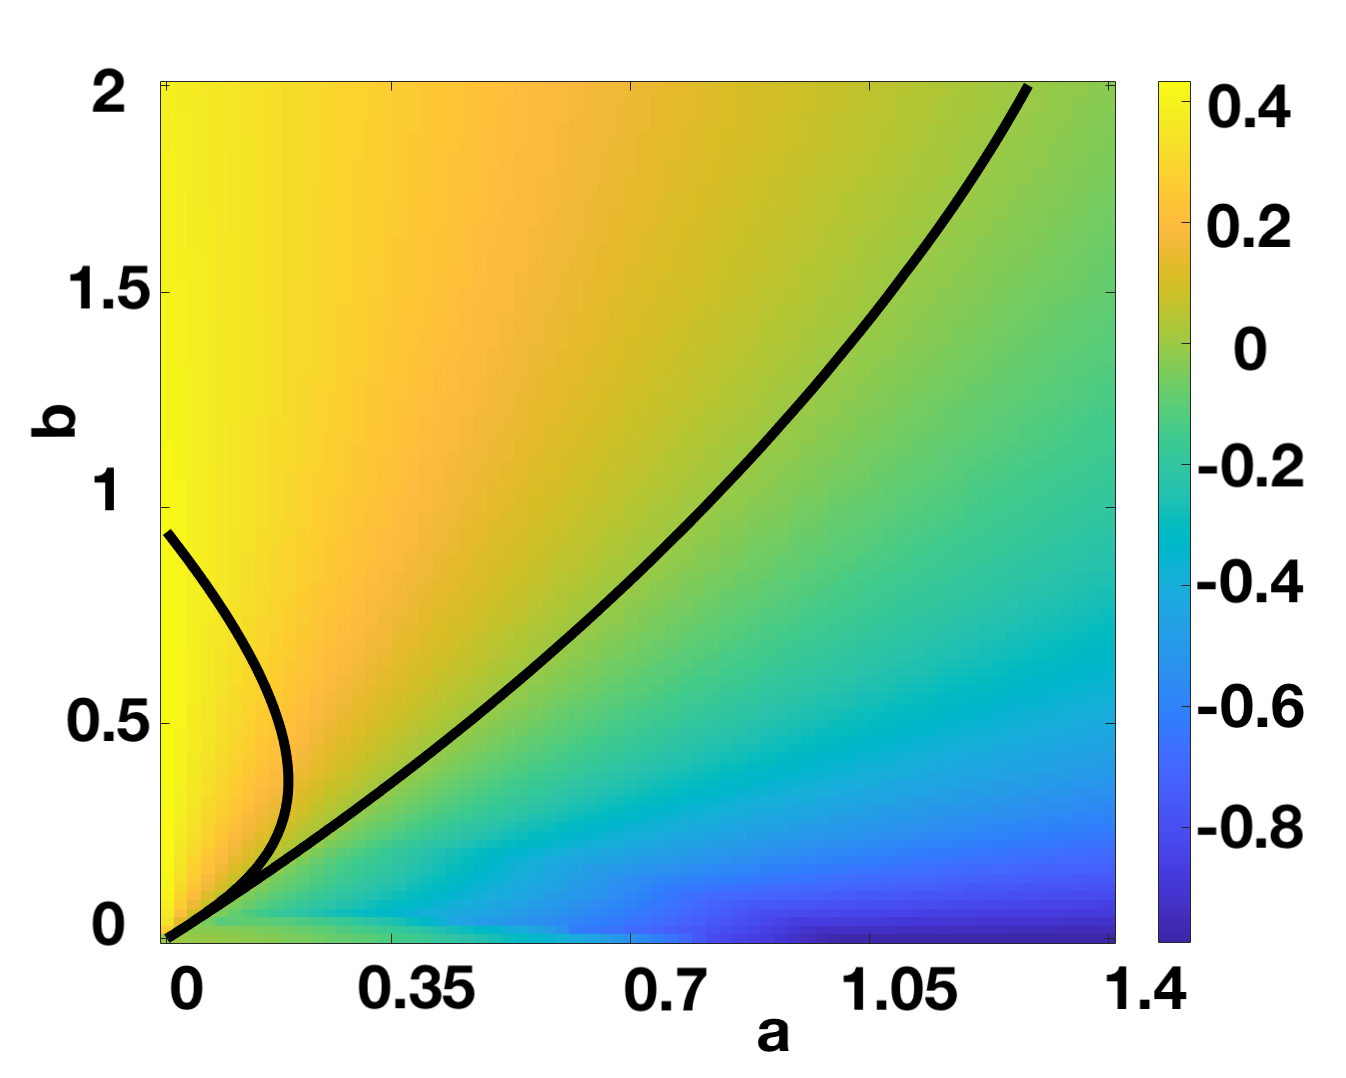
\includegraphics[width=7cm,height=4.75cm]{t1f4.png}
        \caption{Distributed delay with $\sigma=\sigma_{max}\times0.1$.}
        \label{}
    \end{subfigure}
    \caption{Bifurcation diagrams produced for $\tau=0.2$ and $\sigma=\{ \sigma_{max}\times0.99,\sigma_{max}\times0.2,\sigma_{max}\times0.1 \}$, compared with fixed delay case. $\epsilon^2=0.001$. }
    \label{fig:distbif1}
\end{figure}
\begin{figure}[H]
    \centering
    \begin{subfigure}[b]{0.45\textwidth}
        \centering
        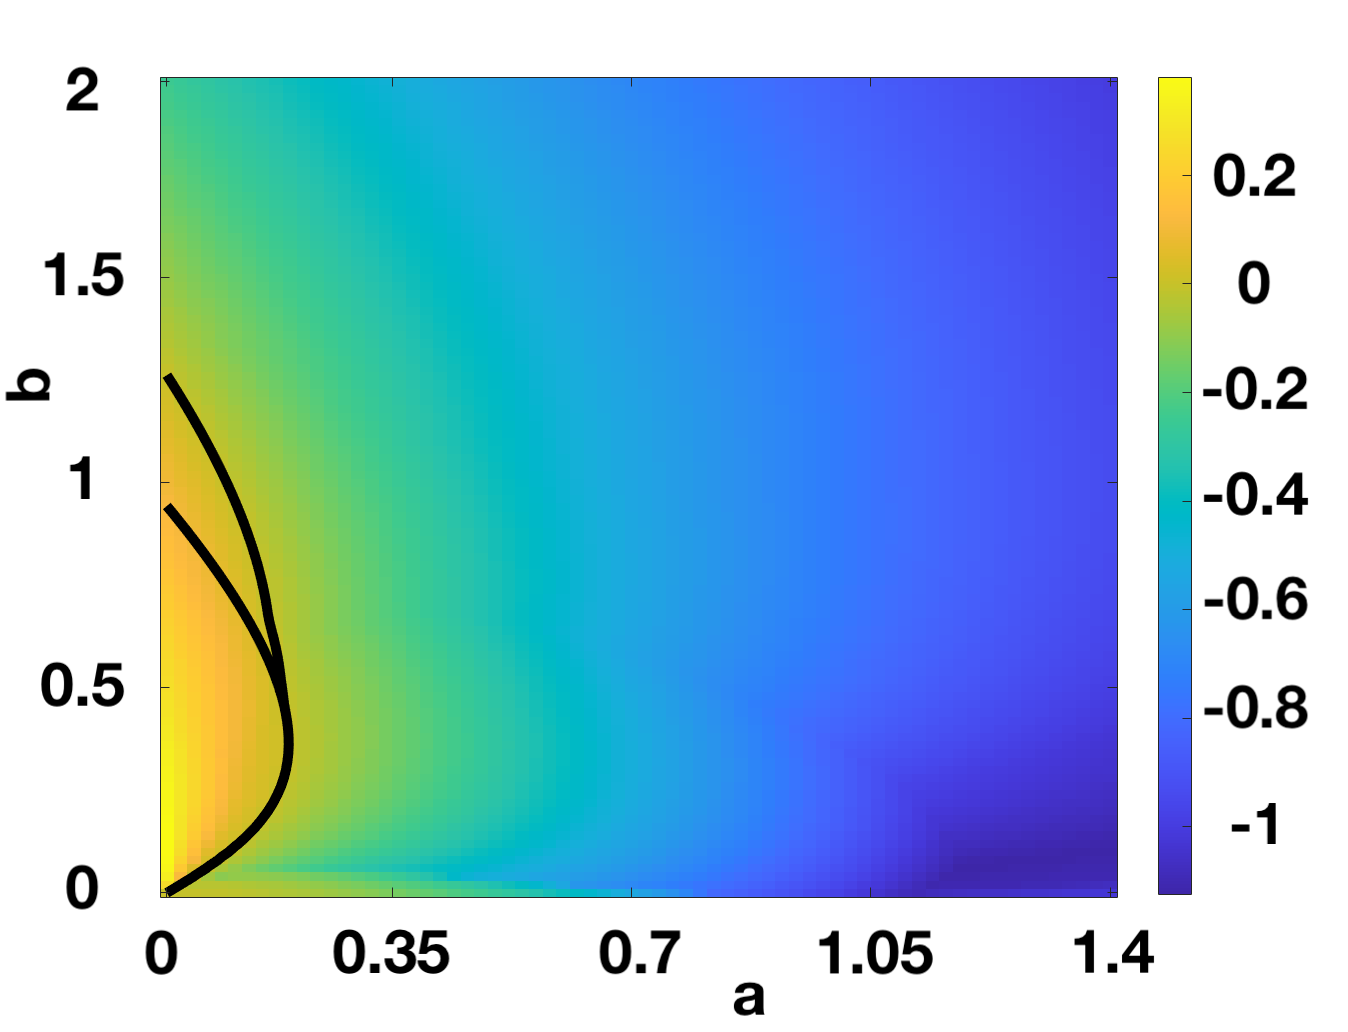
\includegraphics[width=7cm,height=4.75cm]{distbif31.png}
        \caption{Fixed delay case.}
        \label{}
    \end{subfigure}
    \hfill
    \begin{subfigure}[b]{0.45\textwidth}
        \centering
        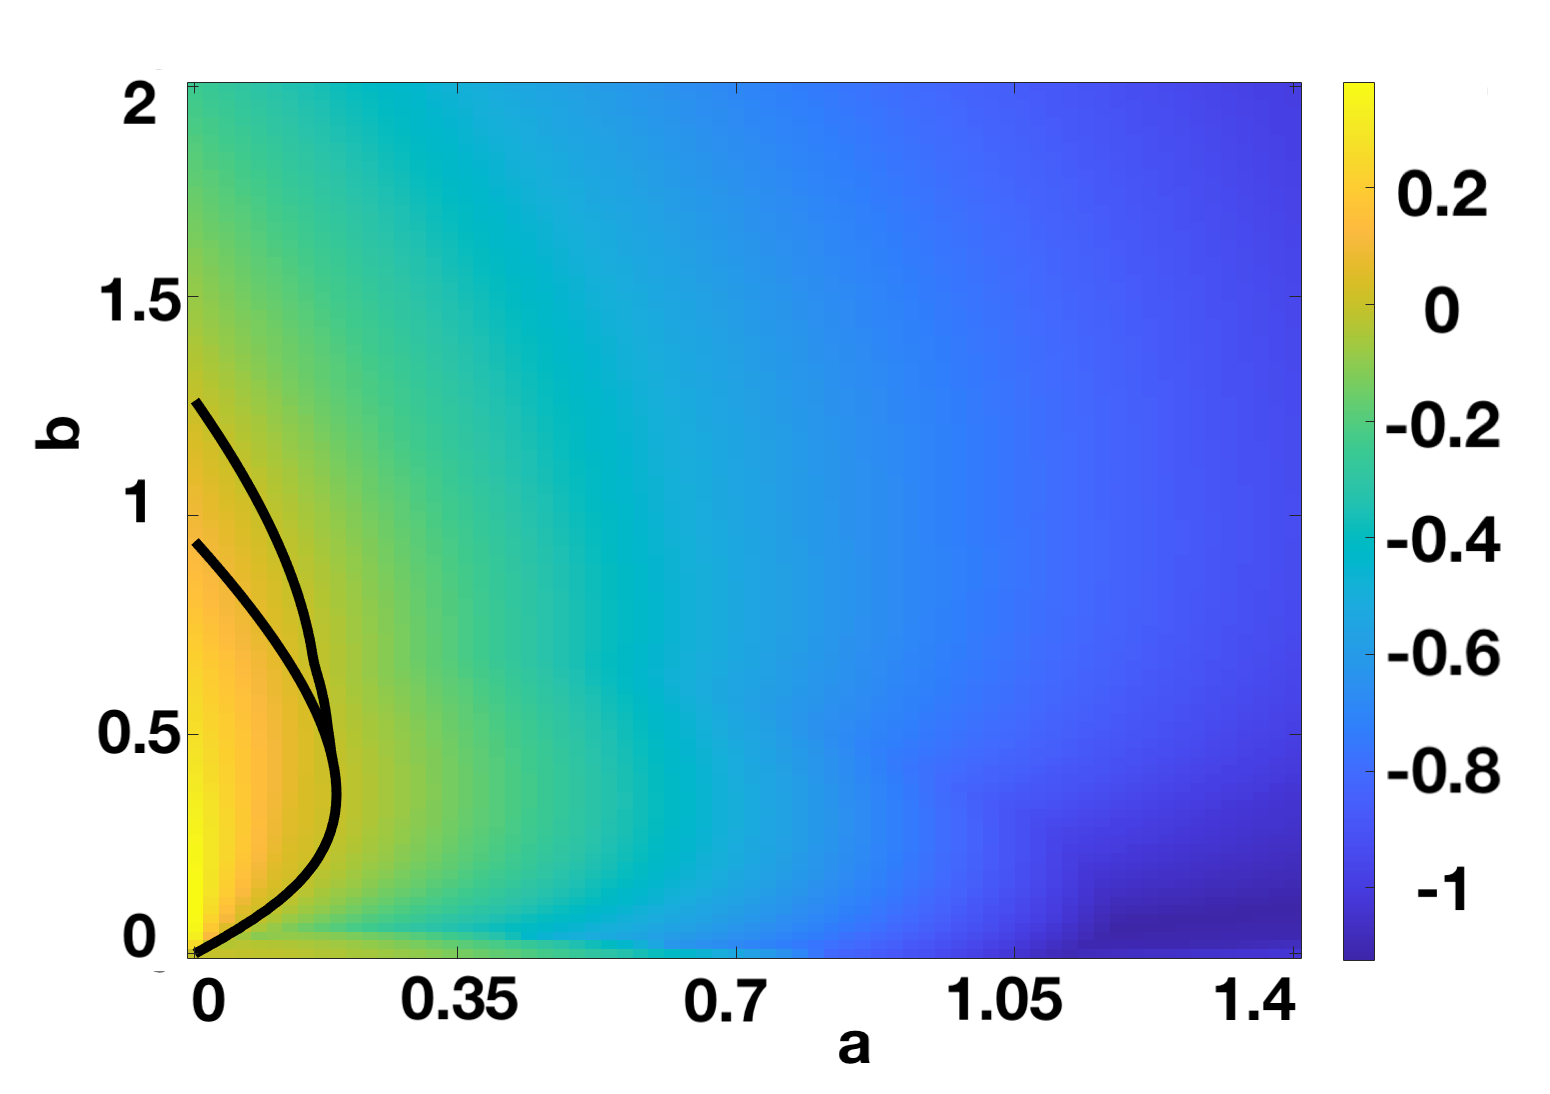
\includegraphics[width=7cm,height=4.75cm]{distbif32.png}
        \caption{Distributed delay with $\sigma=\sigma_{max}\times0.99$.}
        \label{}
    \end{subfigure}
    \hfill
    \begin{subfigure}[b]{0.45\textwidth}
        \centering
        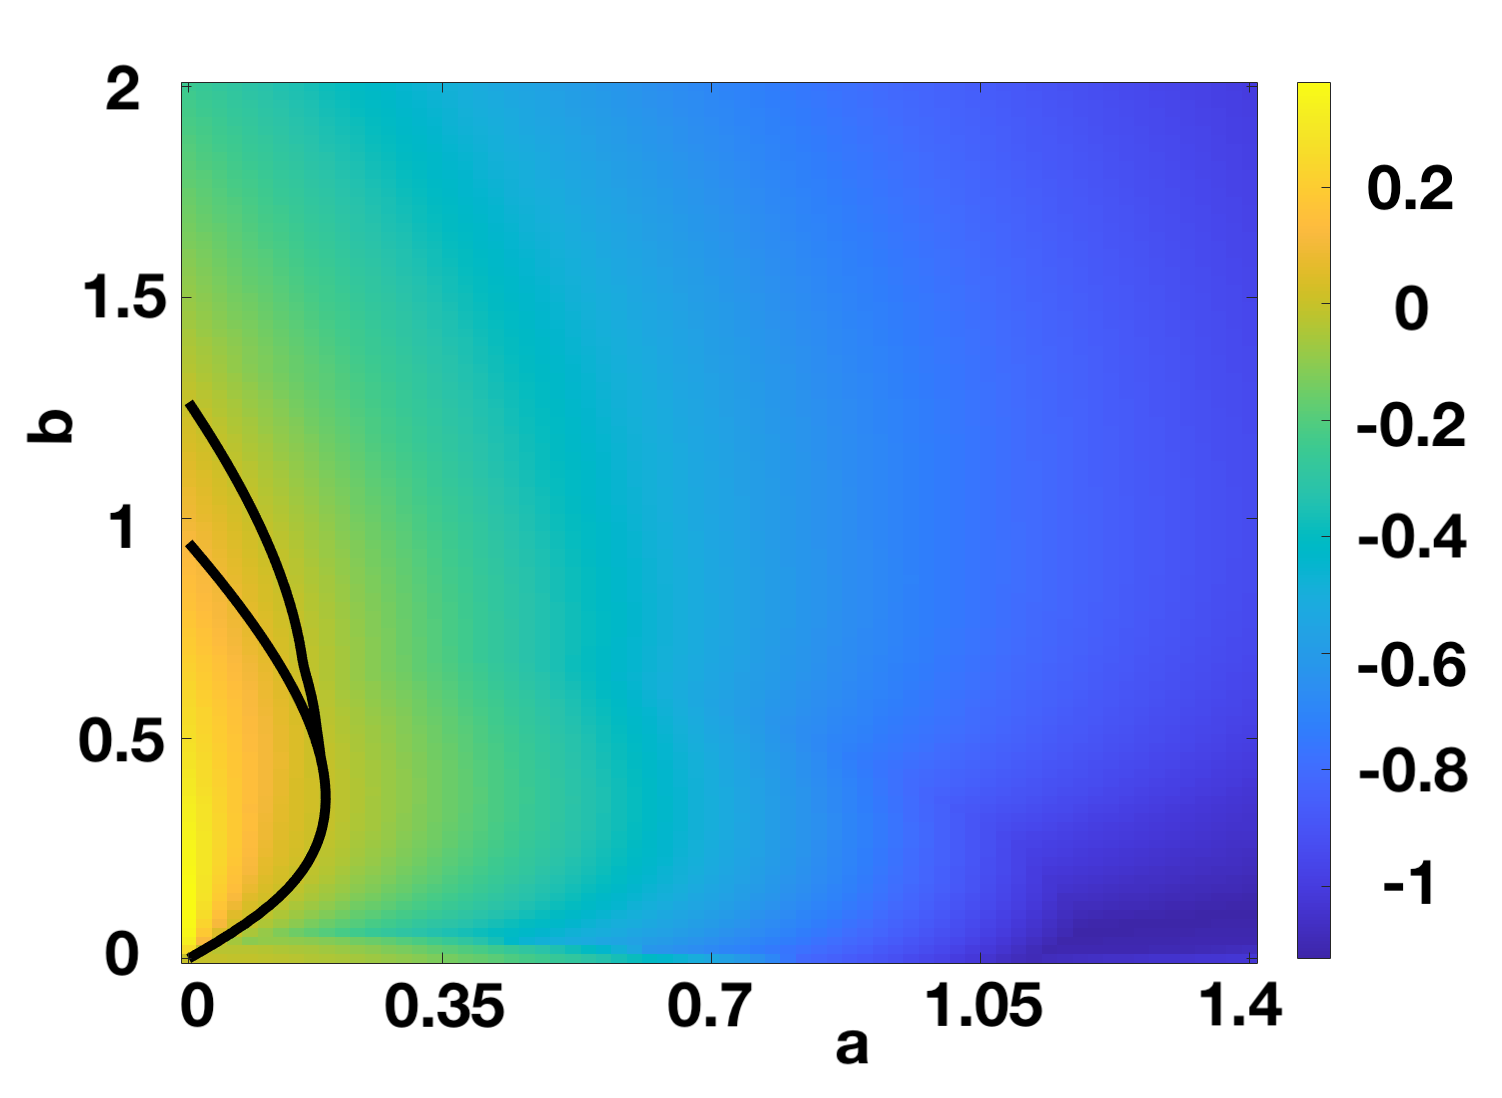
\includegraphics[width=7cm,height=4.75cm]{distbif33.png}
        \caption{Distributed delay with $\sigma=\sigma_{max}\times0.2$.}
        \label{}
    \end{subfigure}
    \hfill
    \begin{subfigure}[b]{0.45\textwidth}
        \centering
        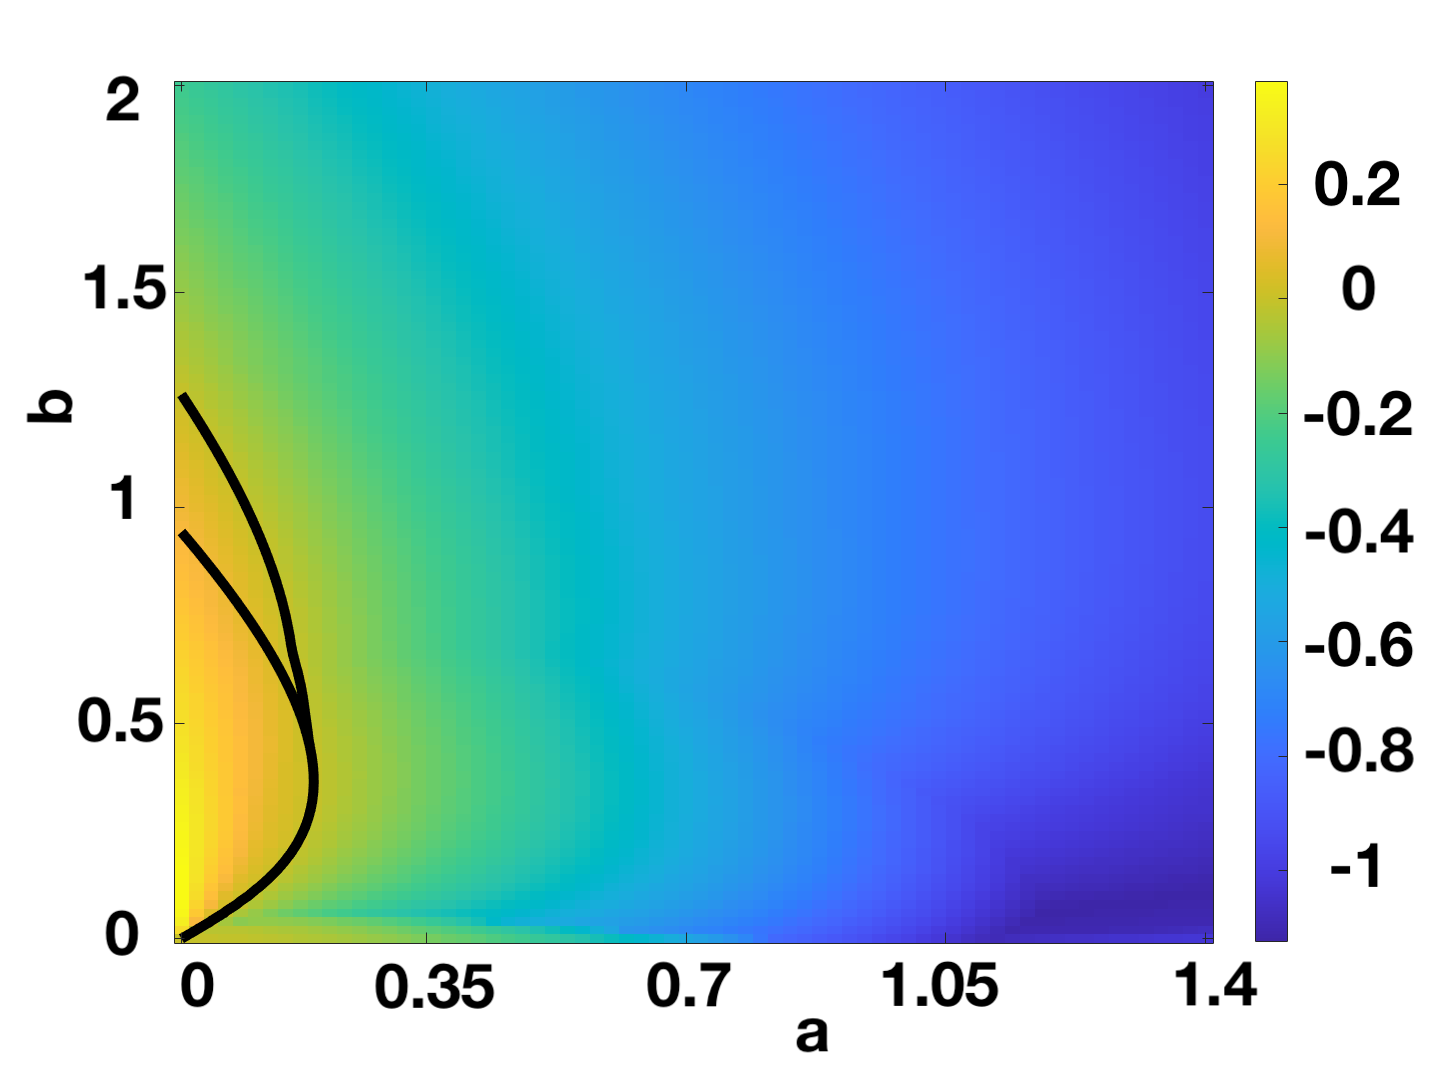
\includegraphics[width=7cm,height=4.75cm]{distbif34.png}
        \caption{Distributed delay with $\sigma=\sigma_{max}\times0.1$.}
        \label{}
    \end{subfigure}
    \caption{Bifurcation diagrams produced for $\tau=0.2$ and $\sigma=\{ \sigma_{max}\times0.99,\sigma_{max}\times0.2,\sigma_{max}\times0.1 \}$, compared with fixed delay case. $\epsilon^2=0.1$.}
    \label{fig:distbif3}
\end{figure}
\begin{figure}[H]
    \centering
    \begin{subfigure}[b]{0.45\textwidth}
        \centering
        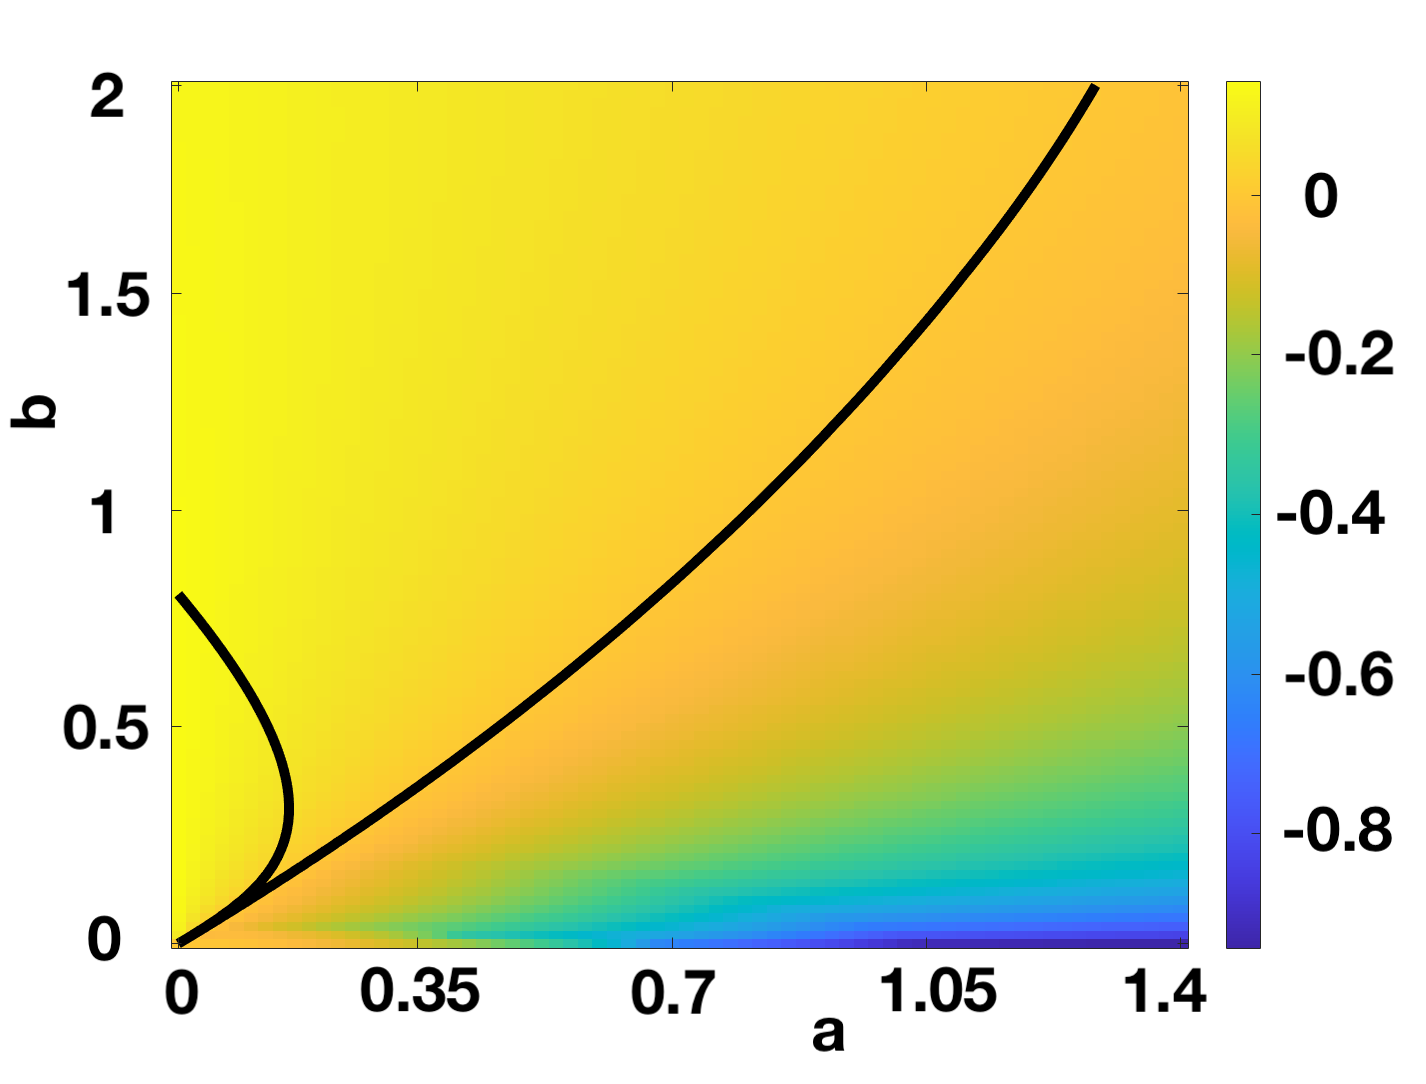
\includegraphics[width=7cm,height=4.75cm]{t2f1.png}
        \caption{Fixed delay case.}
        \label{}
    \end{subfigure}
    \hfill
    \begin{subfigure}[b]{0.45\textwidth}
        \centering
        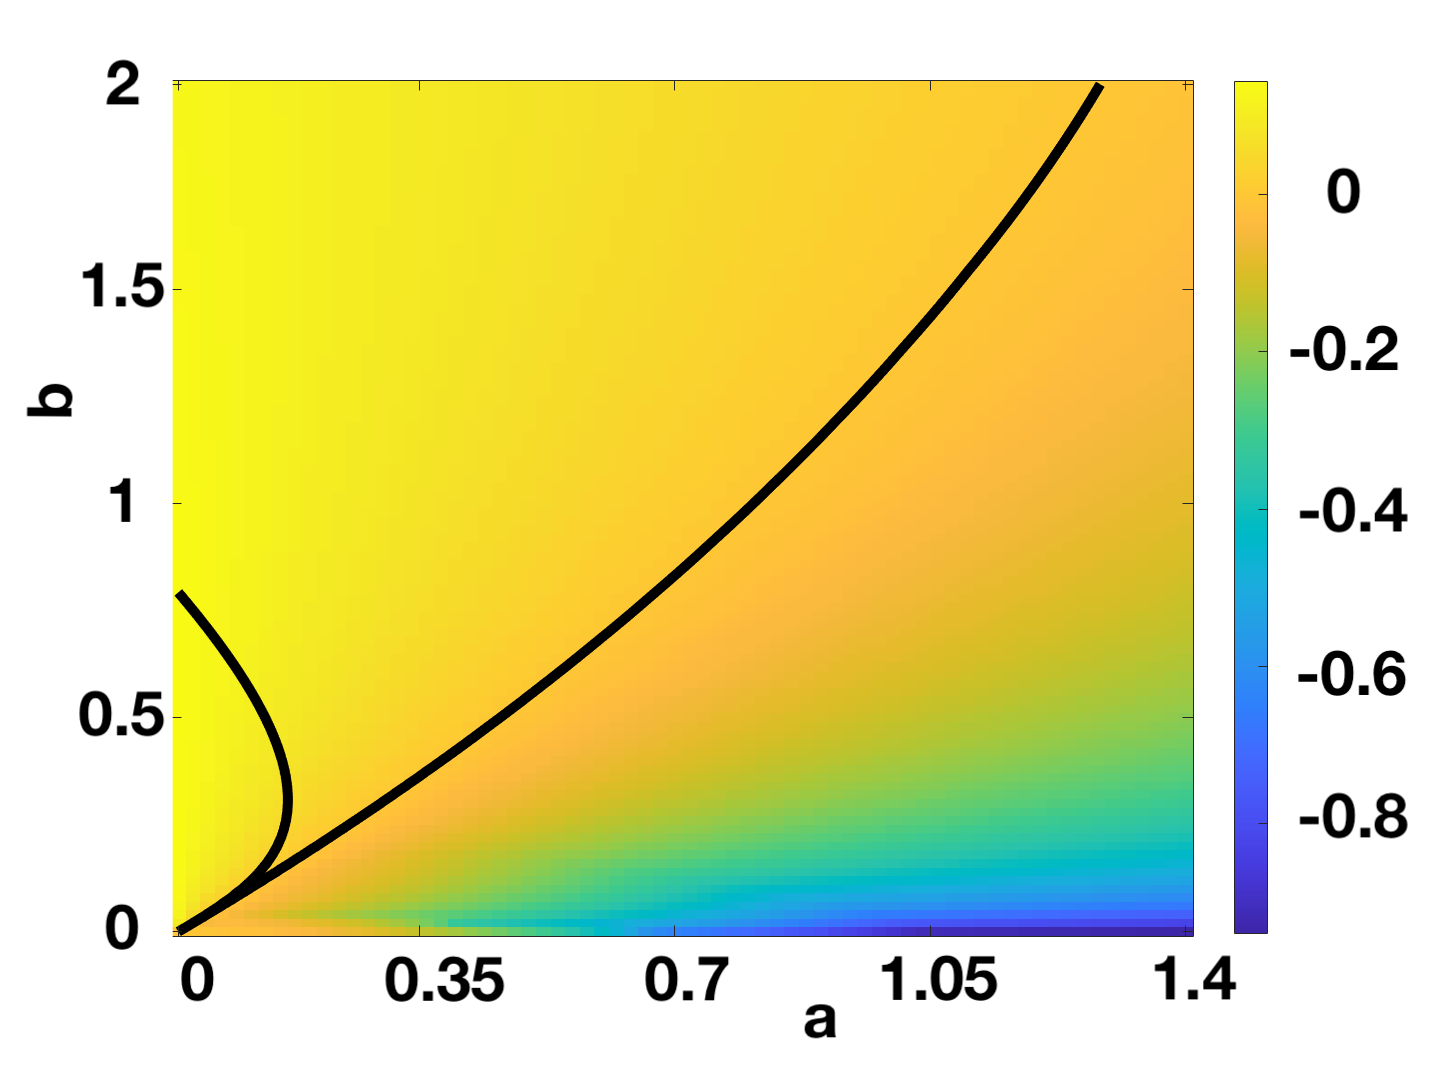
\includegraphics[width=7cm,height=4.75cm]{t2f2.png}
        \caption{Distributed delay with $\sigma=\sigma_{max}\times0.99$.}
        \label{}
    \end{subfigure}
    \hfill
    \begin{subfigure}[b]{0.45\textwidth}
        \centering
        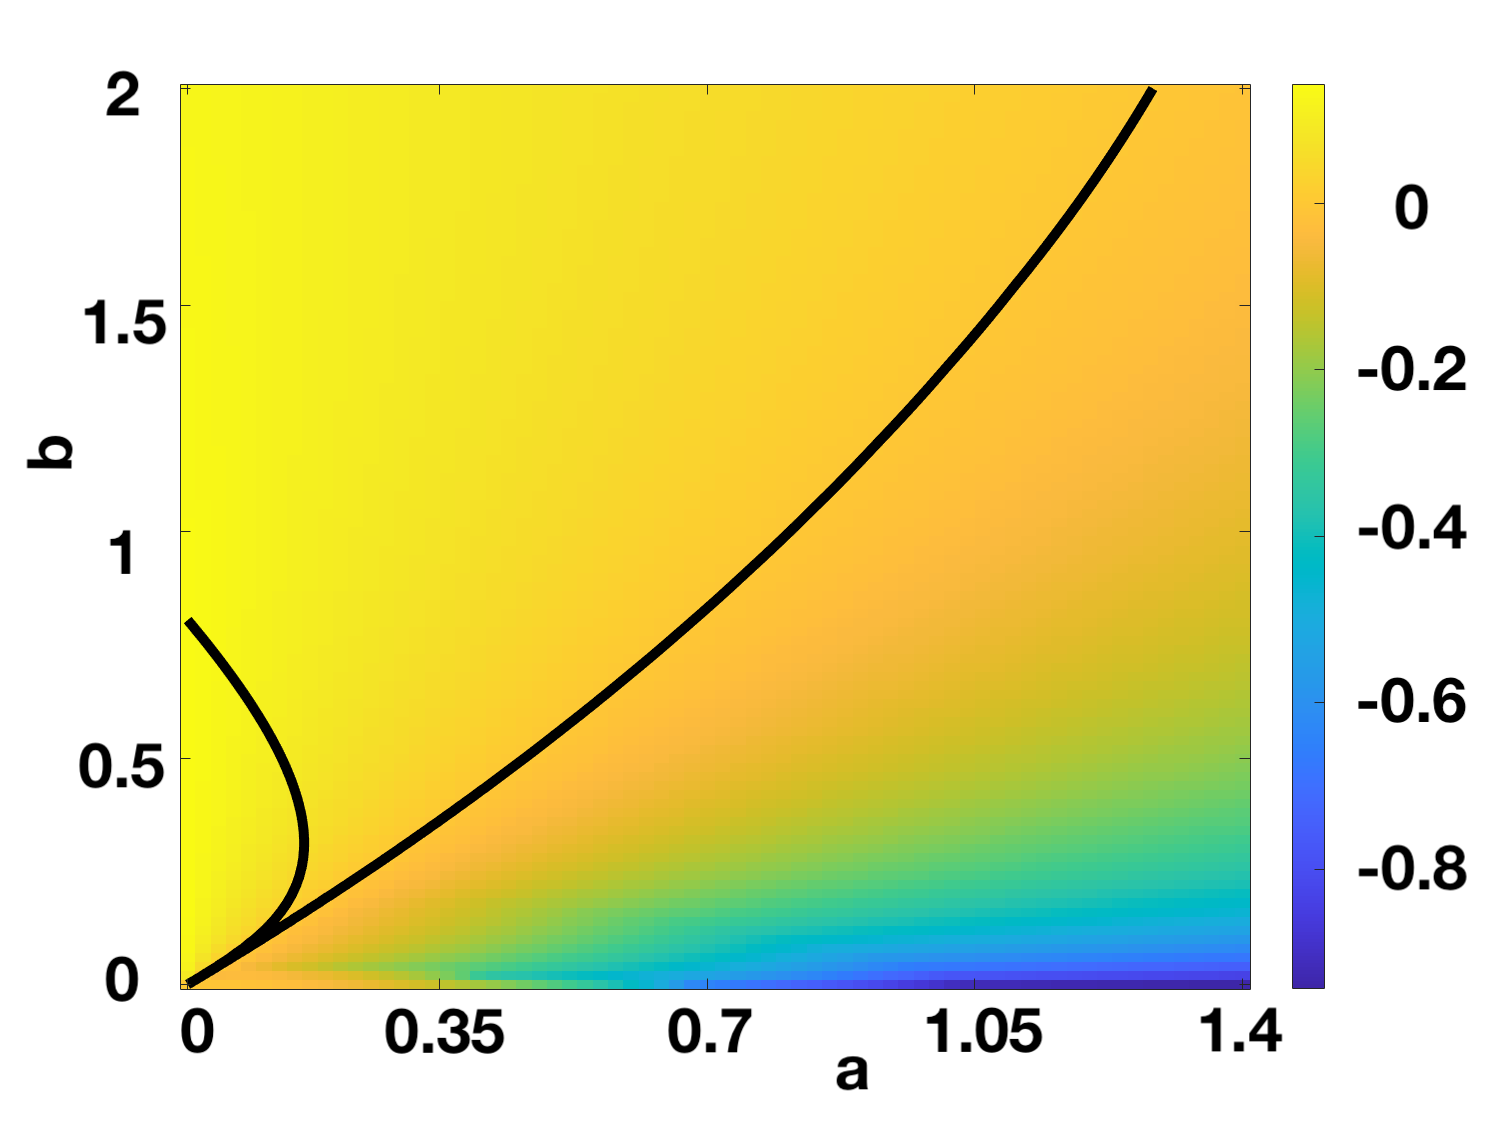
\includegraphics[width=7cm,height=4.75cm]{t2f3.png}
        \caption{Distributed delay with $\sigma=\sigma_{max}\times0.2$.}
        \label{}
    \end{subfigure}
    \hfill
    \begin{subfigure}[b]{0.45\textwidth}
        \centering
        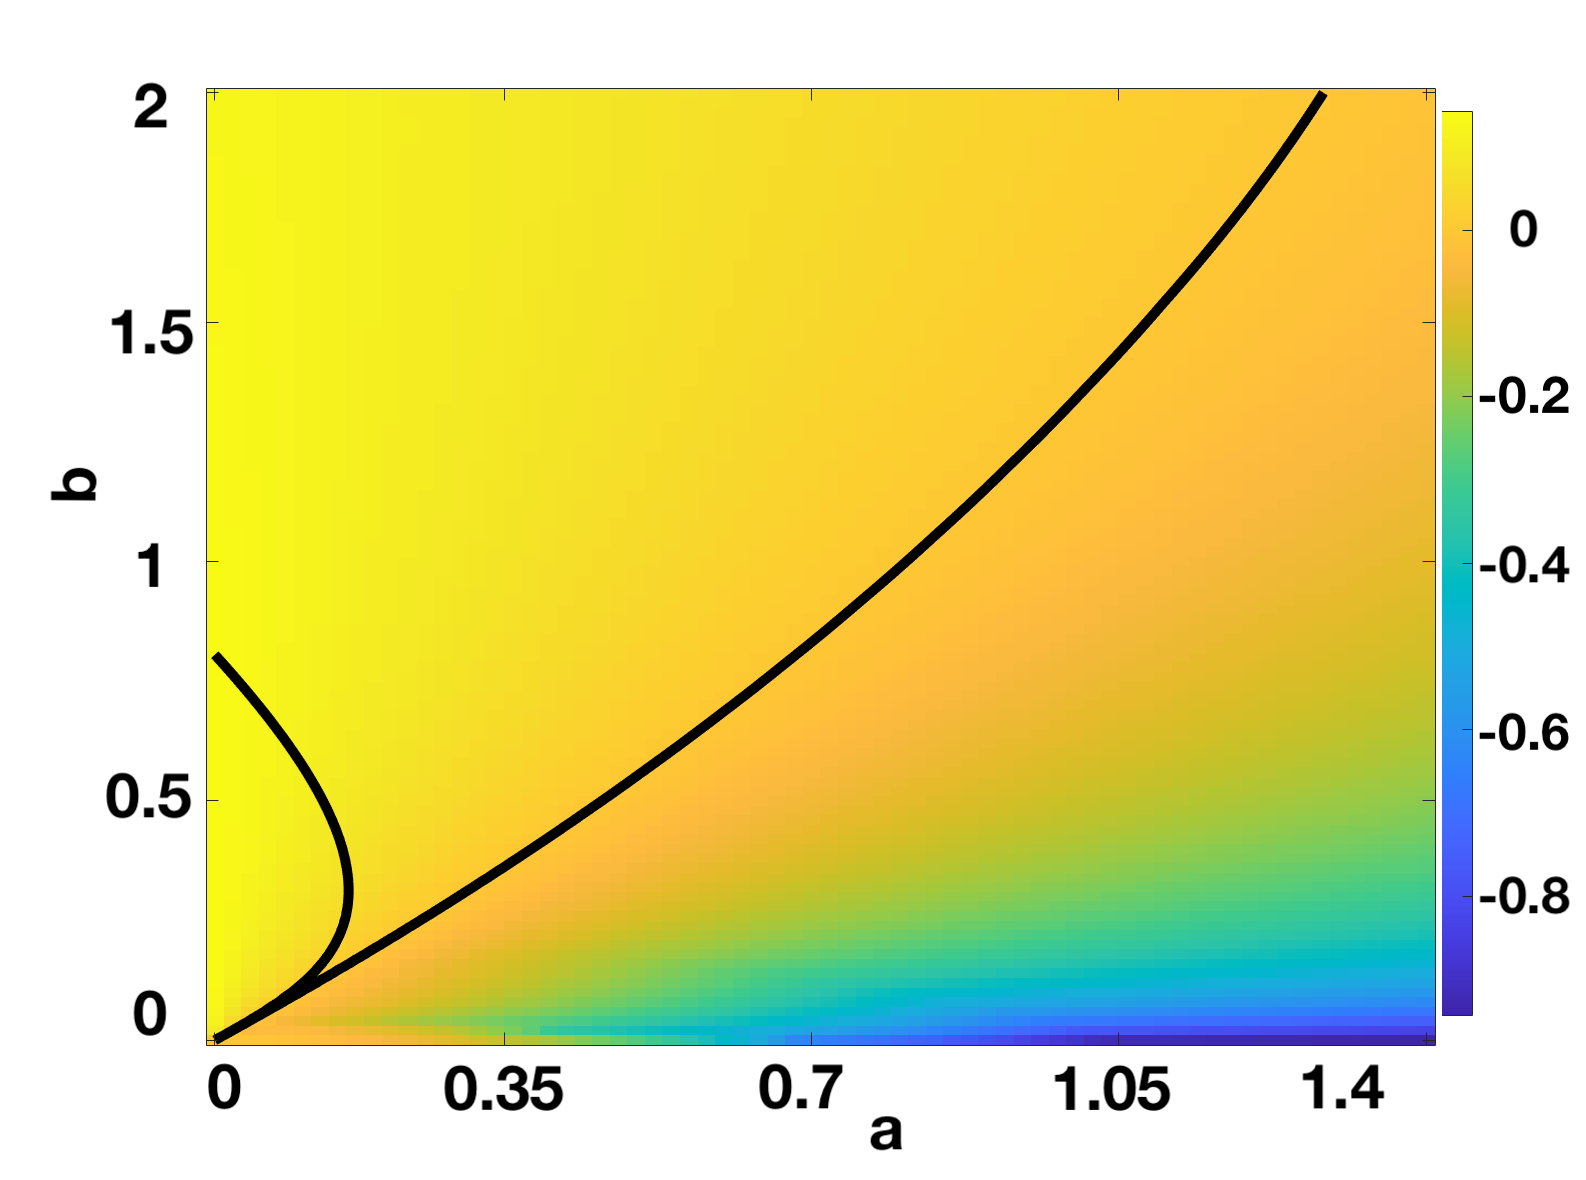
\includegraphics[width=7cm,height=4.75cm]{t2f4.png}
        \caption{Distributed delay with $\sigma=\sigma_{max}\times0.1$.}
        \label{}
    \end{subfigure}
    \caption{Bifurcation diagrams produced for $\tau=1$ and $\sigma=\{ \sigma_{max}\times0.99,\sigma_{max}\times0.2,\sigma_{max}\times0.1 \}$, compared with fixed delay case. $\epsilon^2=0.001$.}
    \label{fig:distbif2}
\end{figure}
\begin{figure}[H]
    \centering
    \begin{subfigure}[b]{0.45\textwidth}
        \centering
        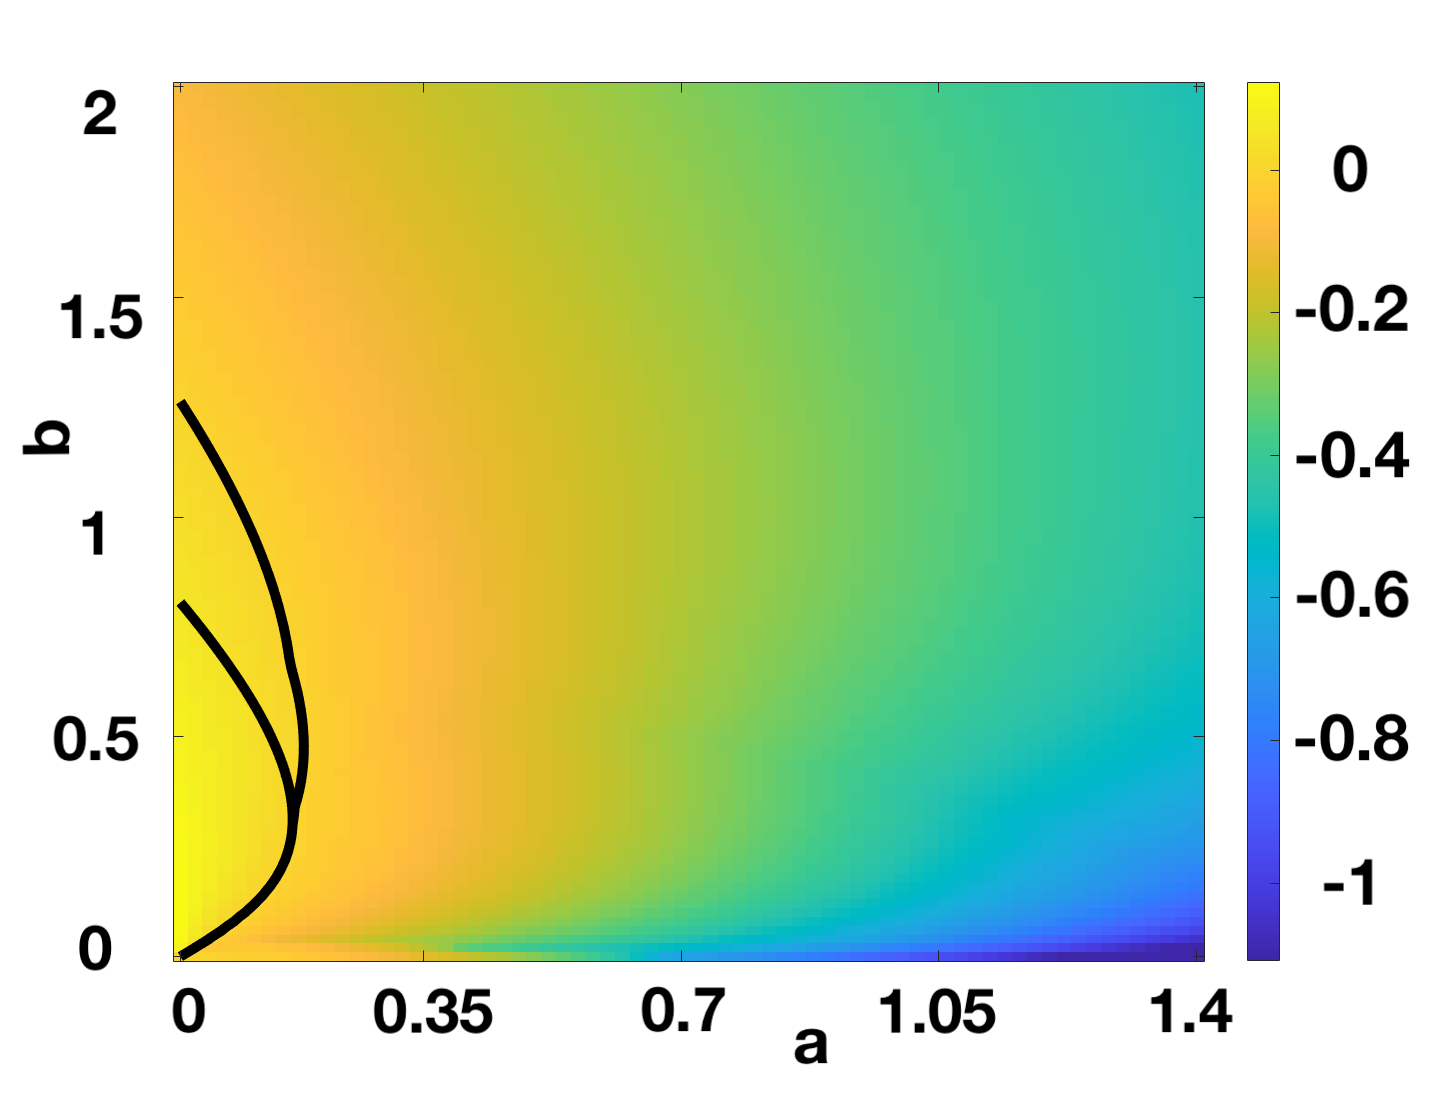
\includegraphics[width=7cm,height=4.75cm]{distbif41.png}
        \caption{Fixed delay case.}
        \label{}
    \end{subfigure}
    \hfill
    \begin{subfigure}[b]{0.45\textwidth}
        \centering
        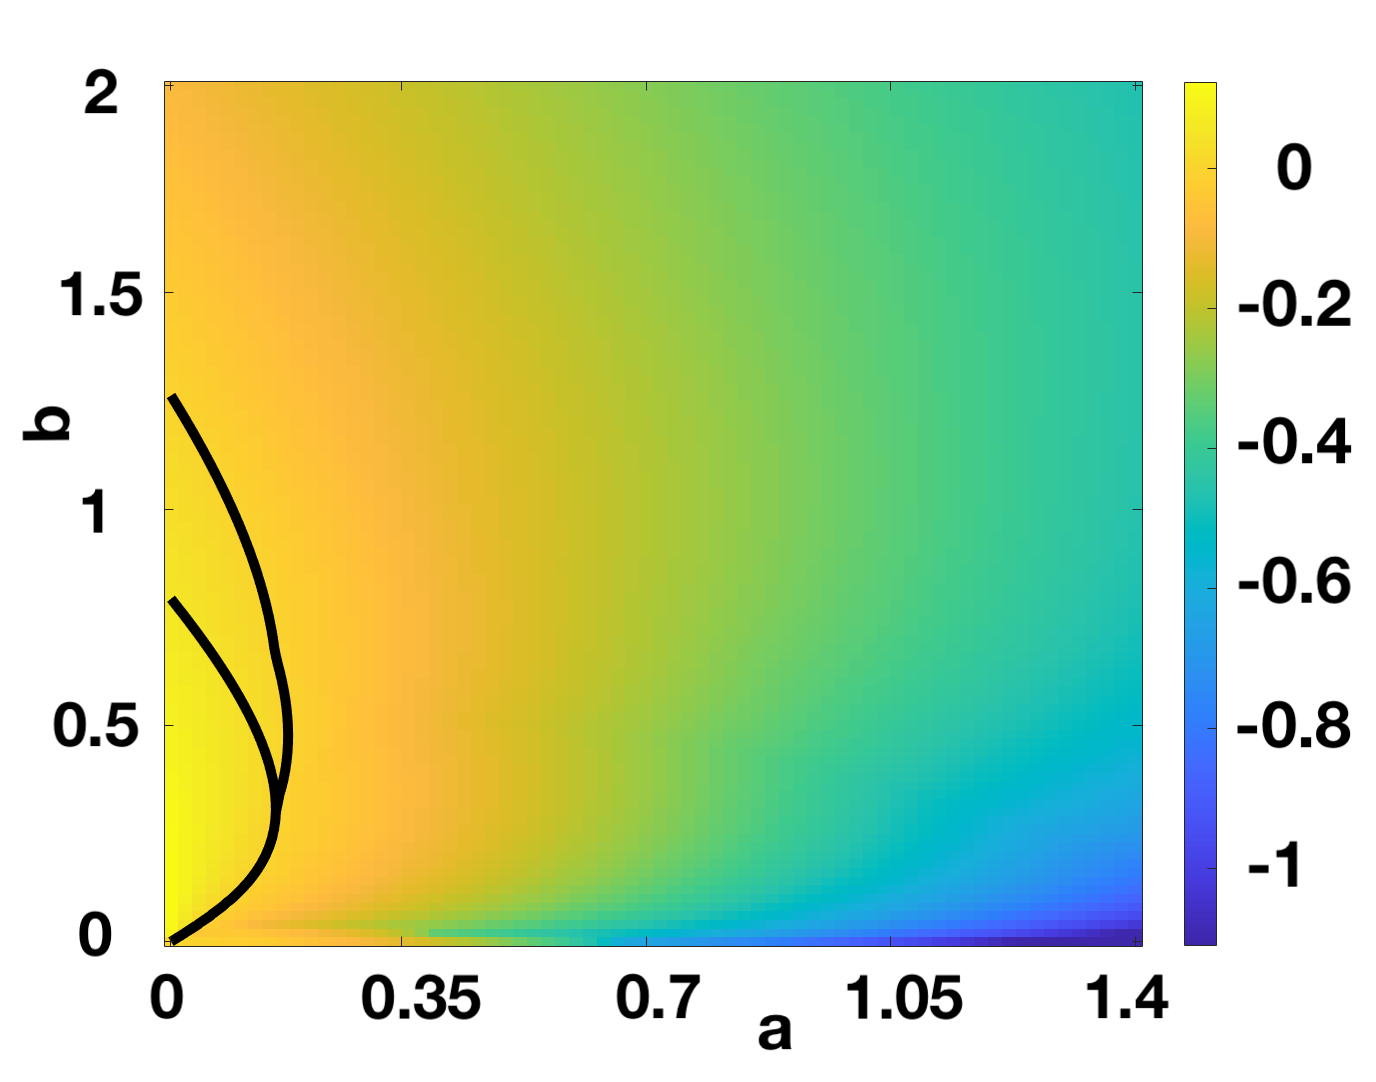
\includegraphics[width=7cm,height=4.75cm]{distbif42.png}
        \caption{Distributed delay with $\sigma=\sigma_{max}\times0.99$.}
        \label{}
    \end{subfigure}
    \hfill
    \begin{subfigure}[b]{0.45\textwidth}
        \centering
        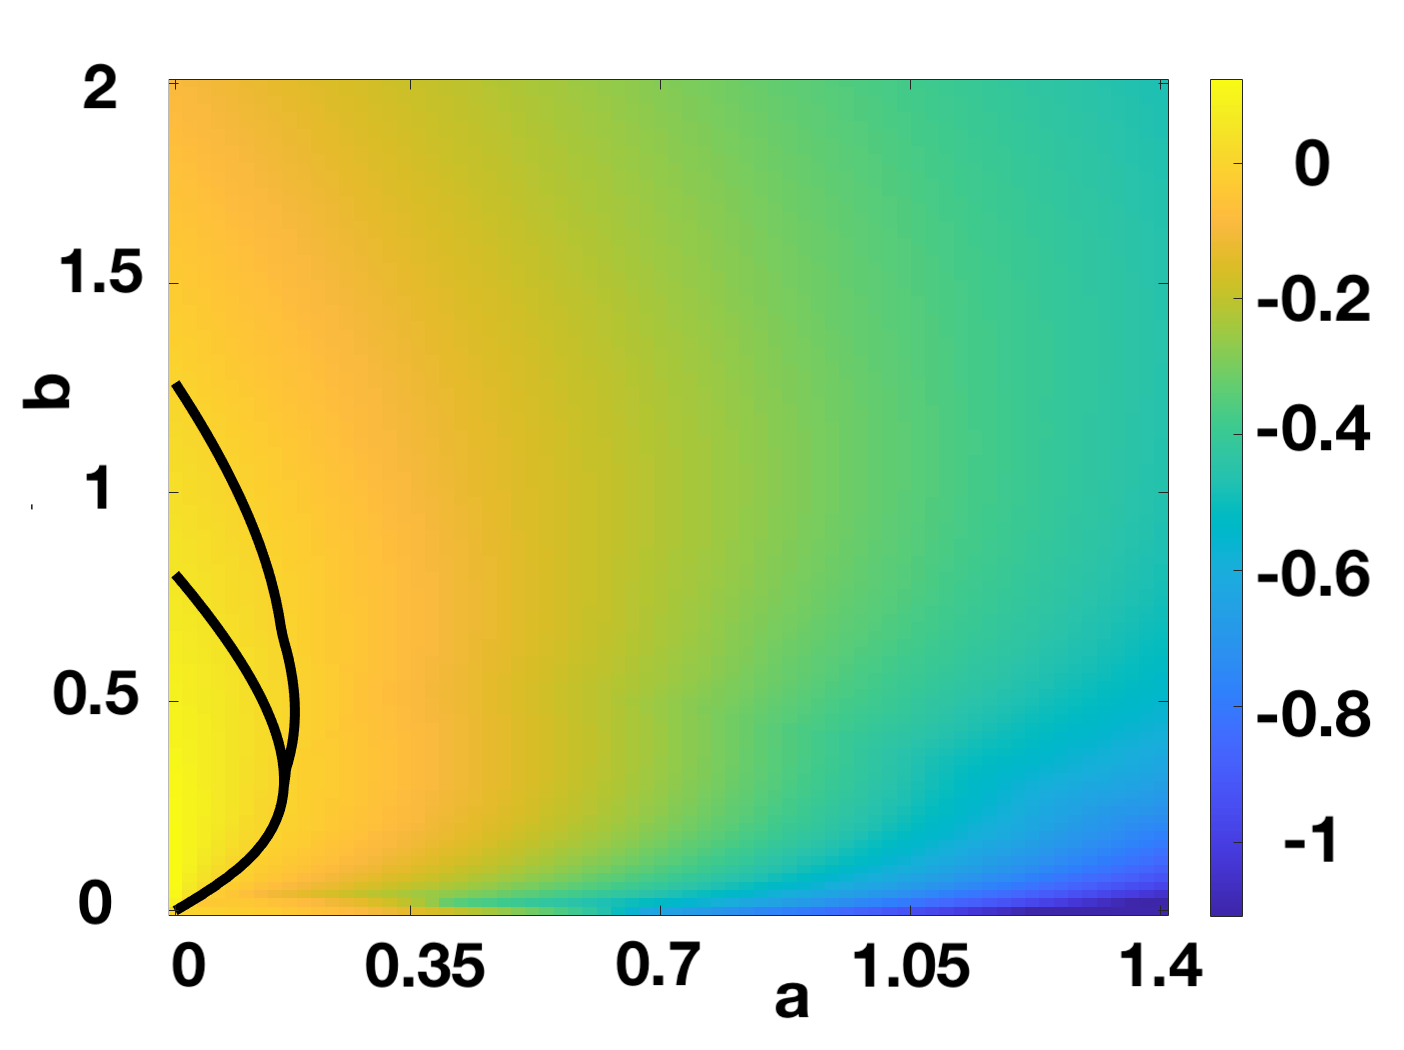
\includegraphics[width=7cm,height=4.75cm]{distbif43.png}
        \caption{Distributed delay with $\sigma=\sigma_{max}\times0.2$.}
        \label{}
    \end{subfigure}
    \hfill
    \begin{subfigure}[b]{0.45\textwidth}
        \centering
        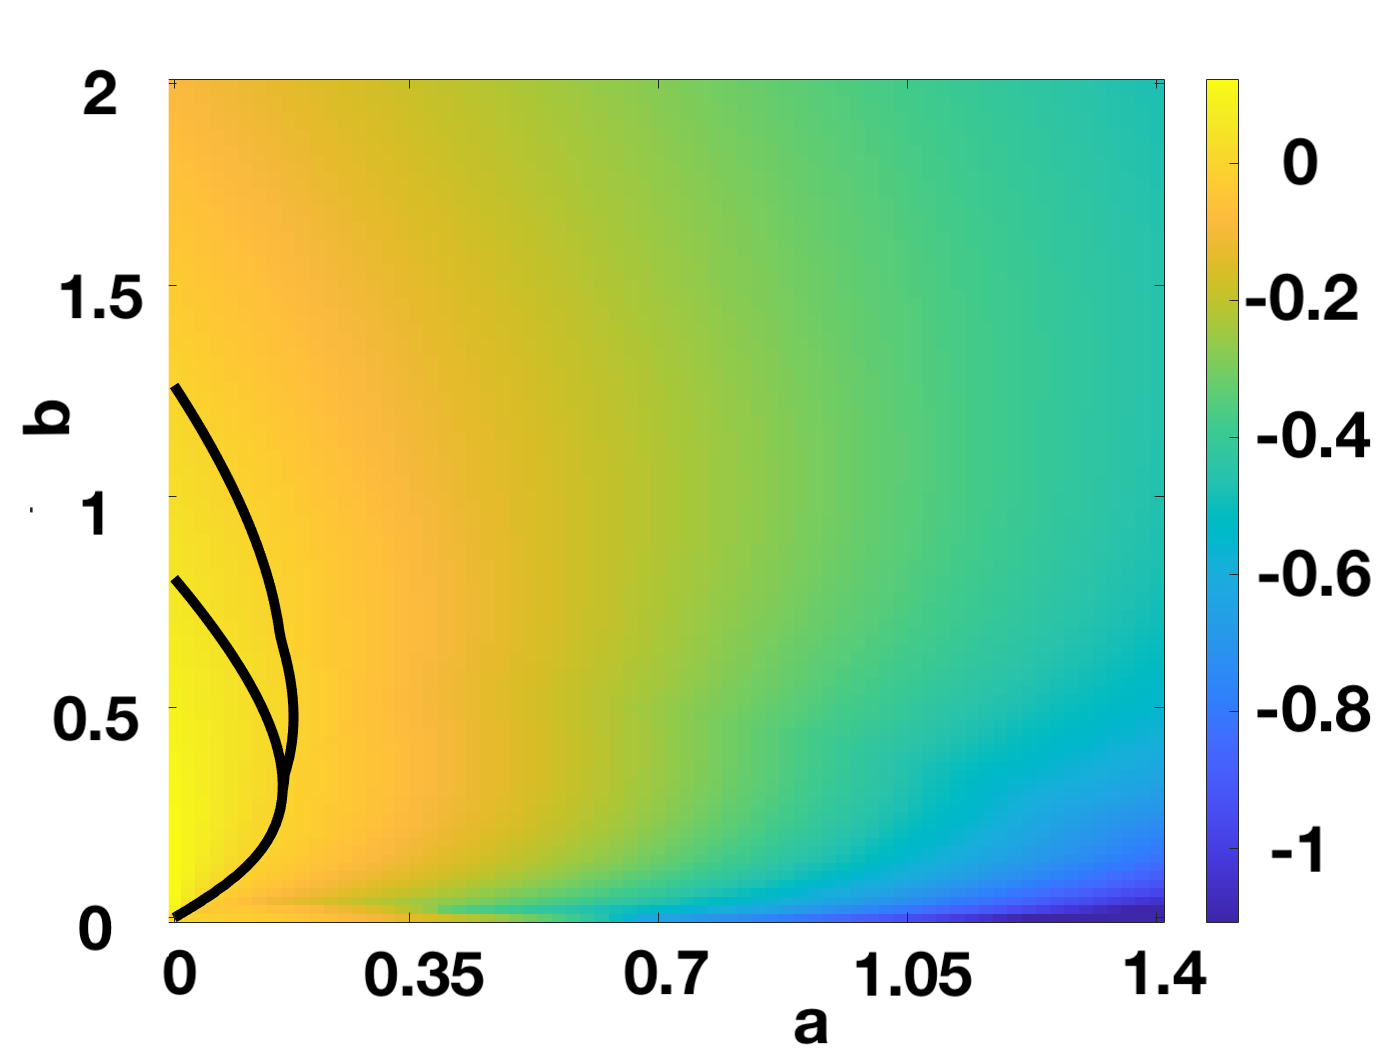
\includegraphics[width=7cm,height=4.75cm]{distbif44.png}
        \caption{Distributed delay with $\sigma=\sigma_{max}\times0.1$.}
        \label{}
    \end{subfigure}
    \caption{Bifurcation diagrams produced for $\tau=1$ and $\sigma=\{ \sigma_{max}\times0.99,\sigma_{max}\times0.2,\sigma_{max}\times0.1 \}$, compared with fixed delay case. $\epsilon^2=0.1$.}
    \label{fig:distbif4}
\end{figure}

We see that, for $\tau=0.2$, $|\max_k(\Re(\lambda_k))|$ is larger than that of $\tau=1$ for both $\epsilon^2$ values and all $\sigma$ values plotted. We also observe that the bifurcation diagrams do not change as $\sigma$ is varied, independent of the diffusion ration used. We therefore expect that for all $(a,b)\in[0,1.4]\times[0,2]$, using a symmetric Gaussian distribution centred at some mean $\tau$ will not effect the time-taken until pattern formation for a fixed delay of $\tau$, irrespective of the standard deviation $\sigma$ of the distribution.


\section{Numerical Results}\label{section:distsim}
Numerical simulations are presented here to confirm the linear theory presented in section \ref{section:distlin}. Through numerical simulation, for various parameter sets $(a,b,\tau,\sigma,\epsilon^2)$, we show that the time taken until pattern formation does not change as $\sigma$ varies for a fixed $(a,b,\tau,\epsilon^2)$, compared to that of the fixed delay case with a time-delay $\tau$.
